\documentclass[a4paper, 14pt,russian]{extarticle}

\usepackage[russian]{babel}
\usepackage[T2A]{fontenc}
\usepackage[utf8]{inputenc}
%Соответствующий математический шрифт для Times new roman
\usepackage{newtxmath}
\usepackage{fontspec} 
%Times new roman
\defaultfontfeatures{Ligatures={TeX},Renderer=Basic} 
\setmainfont[Ligatures={TeX,Historic}]{Times New Roman}

%Геометрия
\usepackage{geometry}
\geometry{top=20mm}
\geometry{bottom=15mm}
\geometry{left=20mm}
\geometry{right=15mm}
\usepackage{setspace}
%Нормальные дроби через запятую
\usepackage{ncccomma}

\newcommand{\changefont}{%
	\fontsize{12}{11}\selectfont
}

%Заголовки
\usepackage{fancyhdr}
\pagestyle{fancy}
\fancyhf{}
%\renewcommand{\sectionmark}[1]{\markright{#1}}
\fancyhead[R]{\changefont \slshape \leftmark}
\fancyhead[L]{\changefont \slshape \rightmark}
%\newcommand{\ssubsection}[1]{\subsection*{#1}
%	\addcontentsline{toc}{subsection}{#1}
%	\markright{#1}{}}
\cfoot{\thepage}

%\полуторный интервал
\setstretch{1.15}
\setlength{\parindent}{1.25cm}

\usepackage{amsmath, amsfonts, mathtools}
\usepackage{physics}
\usepackage{indentfirst}
\usepackage{xcolor}
\usepackage{alltt}
\usepackage{graphicx}
\usepackage{wrapfig}
%Настройка ссылок
\usepackage{hyperref}
%\usepackage{upgreek}
%\renewcommand{\beta}{\upbeta}
\hypersetup{
	colorlinks,
	citecolor=black,
	filecolor=black,
	linkcolor=black,
	urlcolor=black
}
\usepackage{caption}
\DeclareCaptionLabelSeparator{dot}{. }
\captionsetup{justification=centering,labelsep=dot}
\usepackage{titlesec}

%Формат заголовков
\titleformat{\section}{\bfseries\filcenter\Large}{\thesection}{1em}{}
\titleformat{\subsection}{\bfseries\filcenter\large}{\thesubsection}{1em}{}
\titleformat{\subsubsection}{\bfseries\filcenter\normalsize}{\thesubsubsection}{1em}{}

\usepackage{chngcntr}

%Включить в нумерацию картинок раздел
\counterwithin{figure}{section}

%Листинги кода и их стили
\usepackage{listings}
\lstdefinestyle{c++} {
	language=C++,
	breaklines=true,
	frame=single,
	numbers=left,
	basicstyle=\footnotesize\ttfamily,
	keywordstyle=\bfseries\color{green!40!black},
	commentstyle=\itshape\color{purple!40!black},
	identifierstyle=\color{blue},
	backgroundcolor=\color{gray!10!white},
}

\lstdefinestyle{python}{
	language=Python,
	breaklines=true,
	frame=single,
	numbers=left,
	basicstyle=\footnotesize\ttfamily,
	keywordstyle=\bfseries\color{green!40!black},
	frame=lines
	basicstyle=\footnotesize
}

\lstdefinestyle{cmd}{
	breaklines=true,
	frame=single,
	basicstyle=\footnotesize\ttfamily,
	frame=lines
	basicstyle=\footnotesize
}

\begin{document}
	
	\begin{titlepage}
	\newpage
	\begin{center}
		
\includegraphics[width=\textwidth]{png/tit.png}
		Институт информационных и вычислительных технологий \\
			Кафедра управления и интеллектуальных технологий
		\vspace{1.25cm}
	\end{center}
	
	\vspace{1.2em}
	
	\begin{center}
		%\textsc{\textbf{}}
		\begin{spacing}{1}
			{\Large Расчётное задание \linebreak
			По дисциплине <<Теория автоматического управления>> \\}
			\large{\bf<<Анализ нелинейных систем автоматического управления>>}
		\end{spacing}
	\end{center}
	
	\vspace{5em}
	

	\vspace{6em}
	
		\noindent Выполнил студент: Михайловский М.\,Ю. \\
		Группа: А-03-21 \\
		Вариант: 39\\
		Проверила: Сидорова Е.\,Ю.
	
	
	\vspace{\fill}
	
	\begin{center}
		Москва 2024
	\end{center}
	
\end{titlepage}
	\pagenumbering{arabic}
	\setcounter{page}{2}
	\tableofcontents
	\newpage
	
	\section{Постановка задачи}
	\subsection{Исходные данные}
	
	Дана нелинейная система со структурной схемой представленной на рис.~\ref{scheme}. Нелинейный элемент (НЭ) имеет вид двухпозиционного реле с гистерезисом с параметрами $c = 9,\,B=8$ (рис.~\ref{NE}). Передаточные функции имеют следующий вид:
	\begin{align*}
		&W_1(p) = 0,1; \\
		&W_2(p) = \frac{4}{p^2 + 3p + 9}; \\ 
		&W_3(p) = 3p.
	\end{align*}
	
	\begin{figure}[h]
		\centering\includegraphics[width=.8\textwidth]{png/схема.png}
		\caption{Структурная схема нелинейной системы}
		\label{scheme}
	\end{figure}
	\begin{figure}[h]
		\centering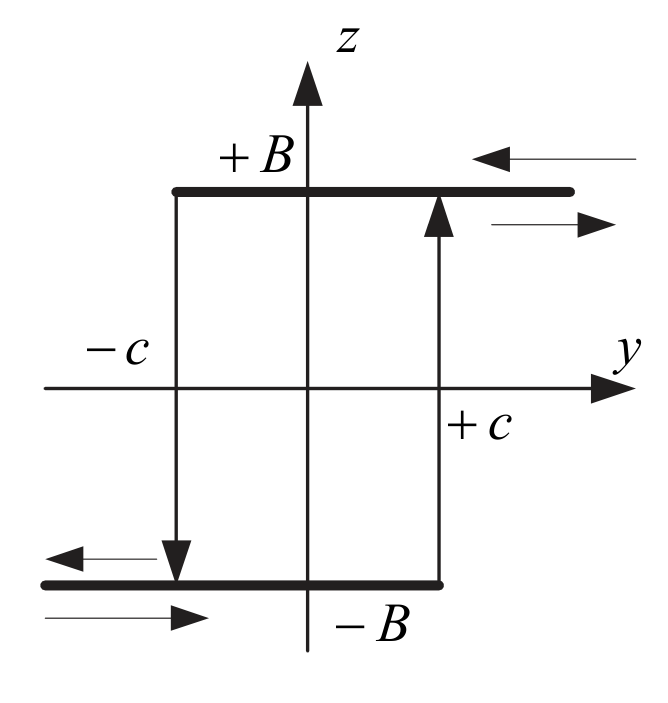
\includegraphics[width=.4\textwidth]{png/НЭ.png}
		\caption{Характеристика НЭ вида двухпозиционное реле с гистерезисом}
		\label{NE}
	\end{figure}
	
	\subsection{План исследования}
	
	\begin{enumerate}
		\item Исследовать структуру фазового портрета нелинейной системы. Для этого определить типы фазовых траекторий в различных областях фазовой плоскости. Найти описание границ данных областей, определить координаты равновесных состояний (особых точек) системы. Построить качественно ожидаемый фазовый портрет системы;
		\item С помощью стандартного ППП построить фазовый портрет системы и сравнить его с ожидаемым, полученным в п. 1. Дать заключение о характере возможных процессов в системе и их устойчивости. Определить устойчивость особых точек, наличие автоколебаний. Для трех фазовых траекторий с начальными условиями $(x_{0_1} \neq 0,\;x'_{0_1}=0)$,  $(x_{0_2} = 0,\;x'_{0_2} 
		\neq 0)$ и $(x_{0_3}\neq 0,\;x'_{0_3}\neq 0)$ привести графики изменения процесса $x(t)$ во времени;
		\item Исследовать влияние ширины петли гистерезиса нелинейного элемента на возникновение автоколебаний в системе. Определить значения параметров $c$ и $h$ НЭ 4, при которых имеют место автоколебания (другие параметры системы остаются неизменными, согласно варианту задания; см. примечание ниже). Для этого найти минимальное значение $\lambda_{\min}$ относительной величины ширины петли гистерезиса $\lambda = \dfrac{h-c}{h}\;(h>c)$, при которой возникают автоколебания. Определить амплитуду и
		период автоколебаний при $\lambda = \lambda_{\min}$;
		\item Определить амплитуду и период автоколебаний при увеличении коэффициента усиления
		$W_1(p)$ в 5 раз и значения $\lambda$ в 2 раза относительно $\lambda$;
		\item Провести исследование автоколебаний в системе приближенным амплитудно-частотным методом (методом Гольдфарба). Для этого привести модель системы исходной структурной схемы (рис. \ref{scheme}) к виду модели Гаммерштейна. Построить амплитудно-фазовую характеристику линейной части и инверсную характеристику $[-z(A)]$ эквивалентного
		комплексного коэффициента усиления нелинейного элемента и дать заключение о возможности возникновения автоколебаний в системе данной структуры и их устойчивости. В случае наличия автоколебаний	определить их параметры;
		
		Исследование провести для трёх случаев:
		\begin{itemize}
			\item системы с исходно заданными номером задания параметрами;
			\item системы с параметрами п. 3 при $\lambda = \lambda_{\min}$;
			\item системы с параметрами п. 4.
		\end{itemize}
		\item Сравнить количественно результаты исследования автоколебаний методом фазовой плоскости в п. 2, 3, 4 и методом Гольдфарба в п. 5.
	\end{enumerate}
	
	\section[Метод фазовой плоскости]{Исследование методом фазовой плоскости}
	\subsection{Получение фазового портрета системы}
	
	Составим уравнения системы в изображениях Лапласа:
	\begin{equation*}
		\begin{cases}
			X(p) = W_1(p)W_2(p)Z(p) = \dfrac{0,4}{p^2+3p+9}Z(p) \\
			Y(p) = W_3(p)X(p) = 3p\cdot X(p) \\
			Z(p) = \varphi(Y(p)-X(p)) = \varphi((3p-1)X(p))
		\end{cases}	
	\end{equation*}
	
	Переходя к оригиналам, получаем:
	\begin{equation}
		\begin{cases}
			x''(t) + 3x'(t) + 9x(t) = 0,4z(t) \\
			y(t) = 3x'(t) \\
			z(t) = \varphi(3x'(t) - x(t))
		\end{cases} \Rightarrow x''+3x'+9x = 0,4\varphi(3x'-x)
		\label{sys_equation}
	\end{equation}

	Аналитически выражение для НЭ задаются следующим образом:
	\begin{equation*}
		z(t) = \varphi(y) = \begin{cases}
			8, &y\geq 9 \\
			8, &-9\geq y \geq 9,\;(z^{-} = 8) \\
			-8, &-9 \geq y \geq 9,\;(z^{-}=-8) \\ 
			-8, &y \leq -9
		\end{cases},\;\text{где } z^{-} = \lim_{\xi\to 0}z(t-\xi)
	\end{equation*}
	
	Перейдём к представлению системы в переменных состояния сделав замену $x'(t) = v(t)$:
	\begin{equation*}
		\begin{cases}
			\dv{x}{t} = v \\
			\dv{v}{t} = 0,4z(3v-x) - 3v - 9x
		\end{cases}
	\end{equation*}
	\begin{equation}
		\begin{cases}
			\dv{x}{t} = v \\
			\dv{v}{t} = \begin{cases}
				3,2-3v-9x, &3v-x\geq 9 \\
				3,2-3v-9x, &-9\geq 3v-x \geq 9,\;(z^{-} = 8) \\
				-3,2-3v-9x, &-9 \geq 3v-x \geq 9,\;(z^{-} = -8) \\ 
				-3,2-3v-9x, &3v-x \leq -9
			\end{cases}
		\end{cases}
		\label{sys_equations}
	\end{equation}
	
	Отсюда полупрямые переключения будут следующие:
	\begin{equation}
		\left[\begin{aligned}
			&3v-x = 9,\,v\geq 0 \\
			&3v-x = -9,\,v\leq 0 
		\end{aligned}\right.
		\label{perekl}
	\end{equation}
	
	Исследуем характер фазовых траекторий для произвольного значения $z(t) = C$. Рассмотрим уравнение (\ref{sys_equation}):
	\begin{equation}
		x''+3x'+9x = C \Rightarrow x'' + 3x' + 9\left(x-\frac{C}{9}\right) = 0
		\label{obsh_ur}
	\end{equation}
	 
	Уравнение (\ref{obsh_ur}) представляет собой сдвинутые по $x$ на $\frac{C}{9}$ вправо фазовые траектории линейной системы, заданной следующим характеристическим уравнением (ХУ):
	\begin{equation*}
		p^2 + 3p + 9 = 0 \Rightarrow p_{1,\,2} = \frac{-3\pm\sqrt{3^2 - 4\cdot9}}{2} = -\frac{3}{2} \pm j\frac{3\sqrt{3}}{2}
	\end{equation*}
	
	Такие корни ХУ соответствуют особой точке типа устойчивый фокус. Переходной процесс будет иметь следующий вид:
	\begin{equation*}
		x(t) = \frac{C}{9} + Ae^{-\frac{3}{2}t}\sin(\frac{3\sqrt{3}}{2}t + \theta)
	\end{equation*}
	Здесь значения $A,\,\theta$ зависят от начальных условий.
	
	НЭ в рассматриваемой системе может принимать 2 значения, поэтому будет два типа фазовых траекторий. 
	
	Пусть $z(t) = 8$ задаёт траектории I типа. Из (\ref{obsh_ur}) видно, что для этого случая $C=0,4\cdot8=3,2$. Тогда $z(t) = -8$ задаёт траектории II типа и $C = -3,2$.
	
	Нарисуем качественно вид траекторий. Учитывая сдвиг по оси $x$ на $\dfrac{C}{9}$, особыми точками будут  $\left(0,35,\,0\right)$ и $\left(-0,35,\,0\right)$ для I и II типа фазовых траекторий соответственно. Полученные траектории показаны на рис. \ref{tracks}.
	
	В результате построения фазового портрета системы получаем следующую картину: рис. \ref{FP}.
	
	
	\noindent{\begin{minipage}{.5\textwidth}
		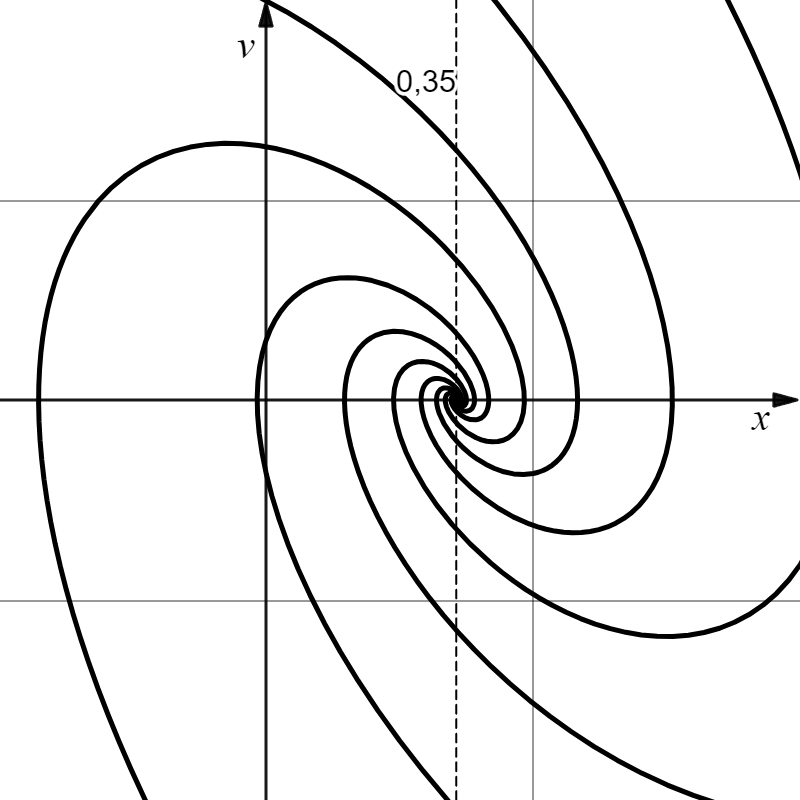
\includegraphics[width=.98\textwidth]{png/траектории1.png}
		\centering I тип
	\end{minipage}
	\begin{minipage}{.5\textwidth}
		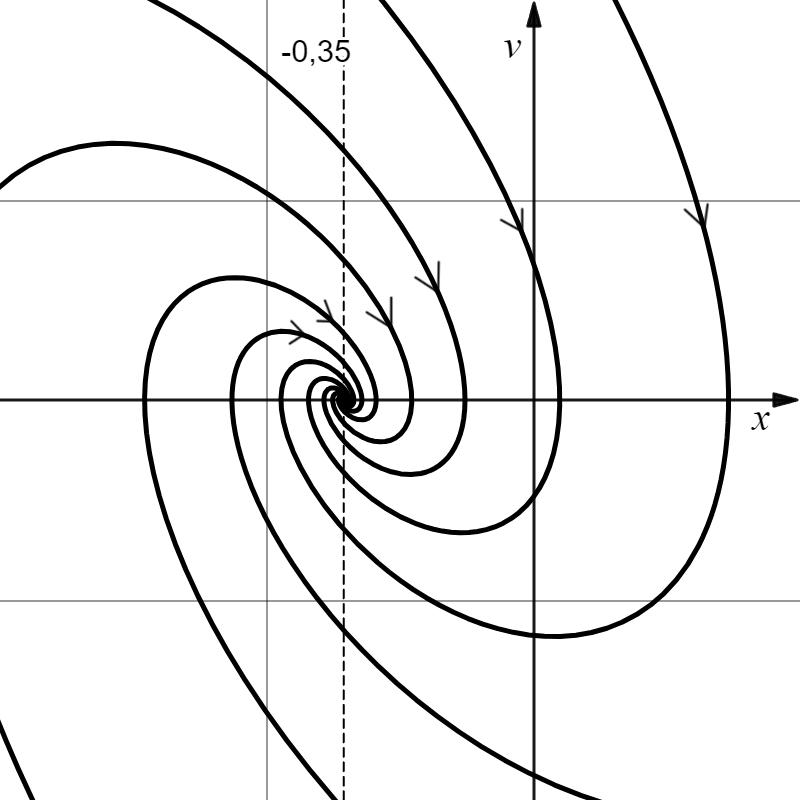
\includegraphics[width=.98\textwidth]{png/траектории2.png}
		\centering II тип
	\end{minipage}
	\captionof{figure}{Фазовые траектории I и II типов}
	\label{tracks}}
	
	
	\begin{figure}[h]
		\centering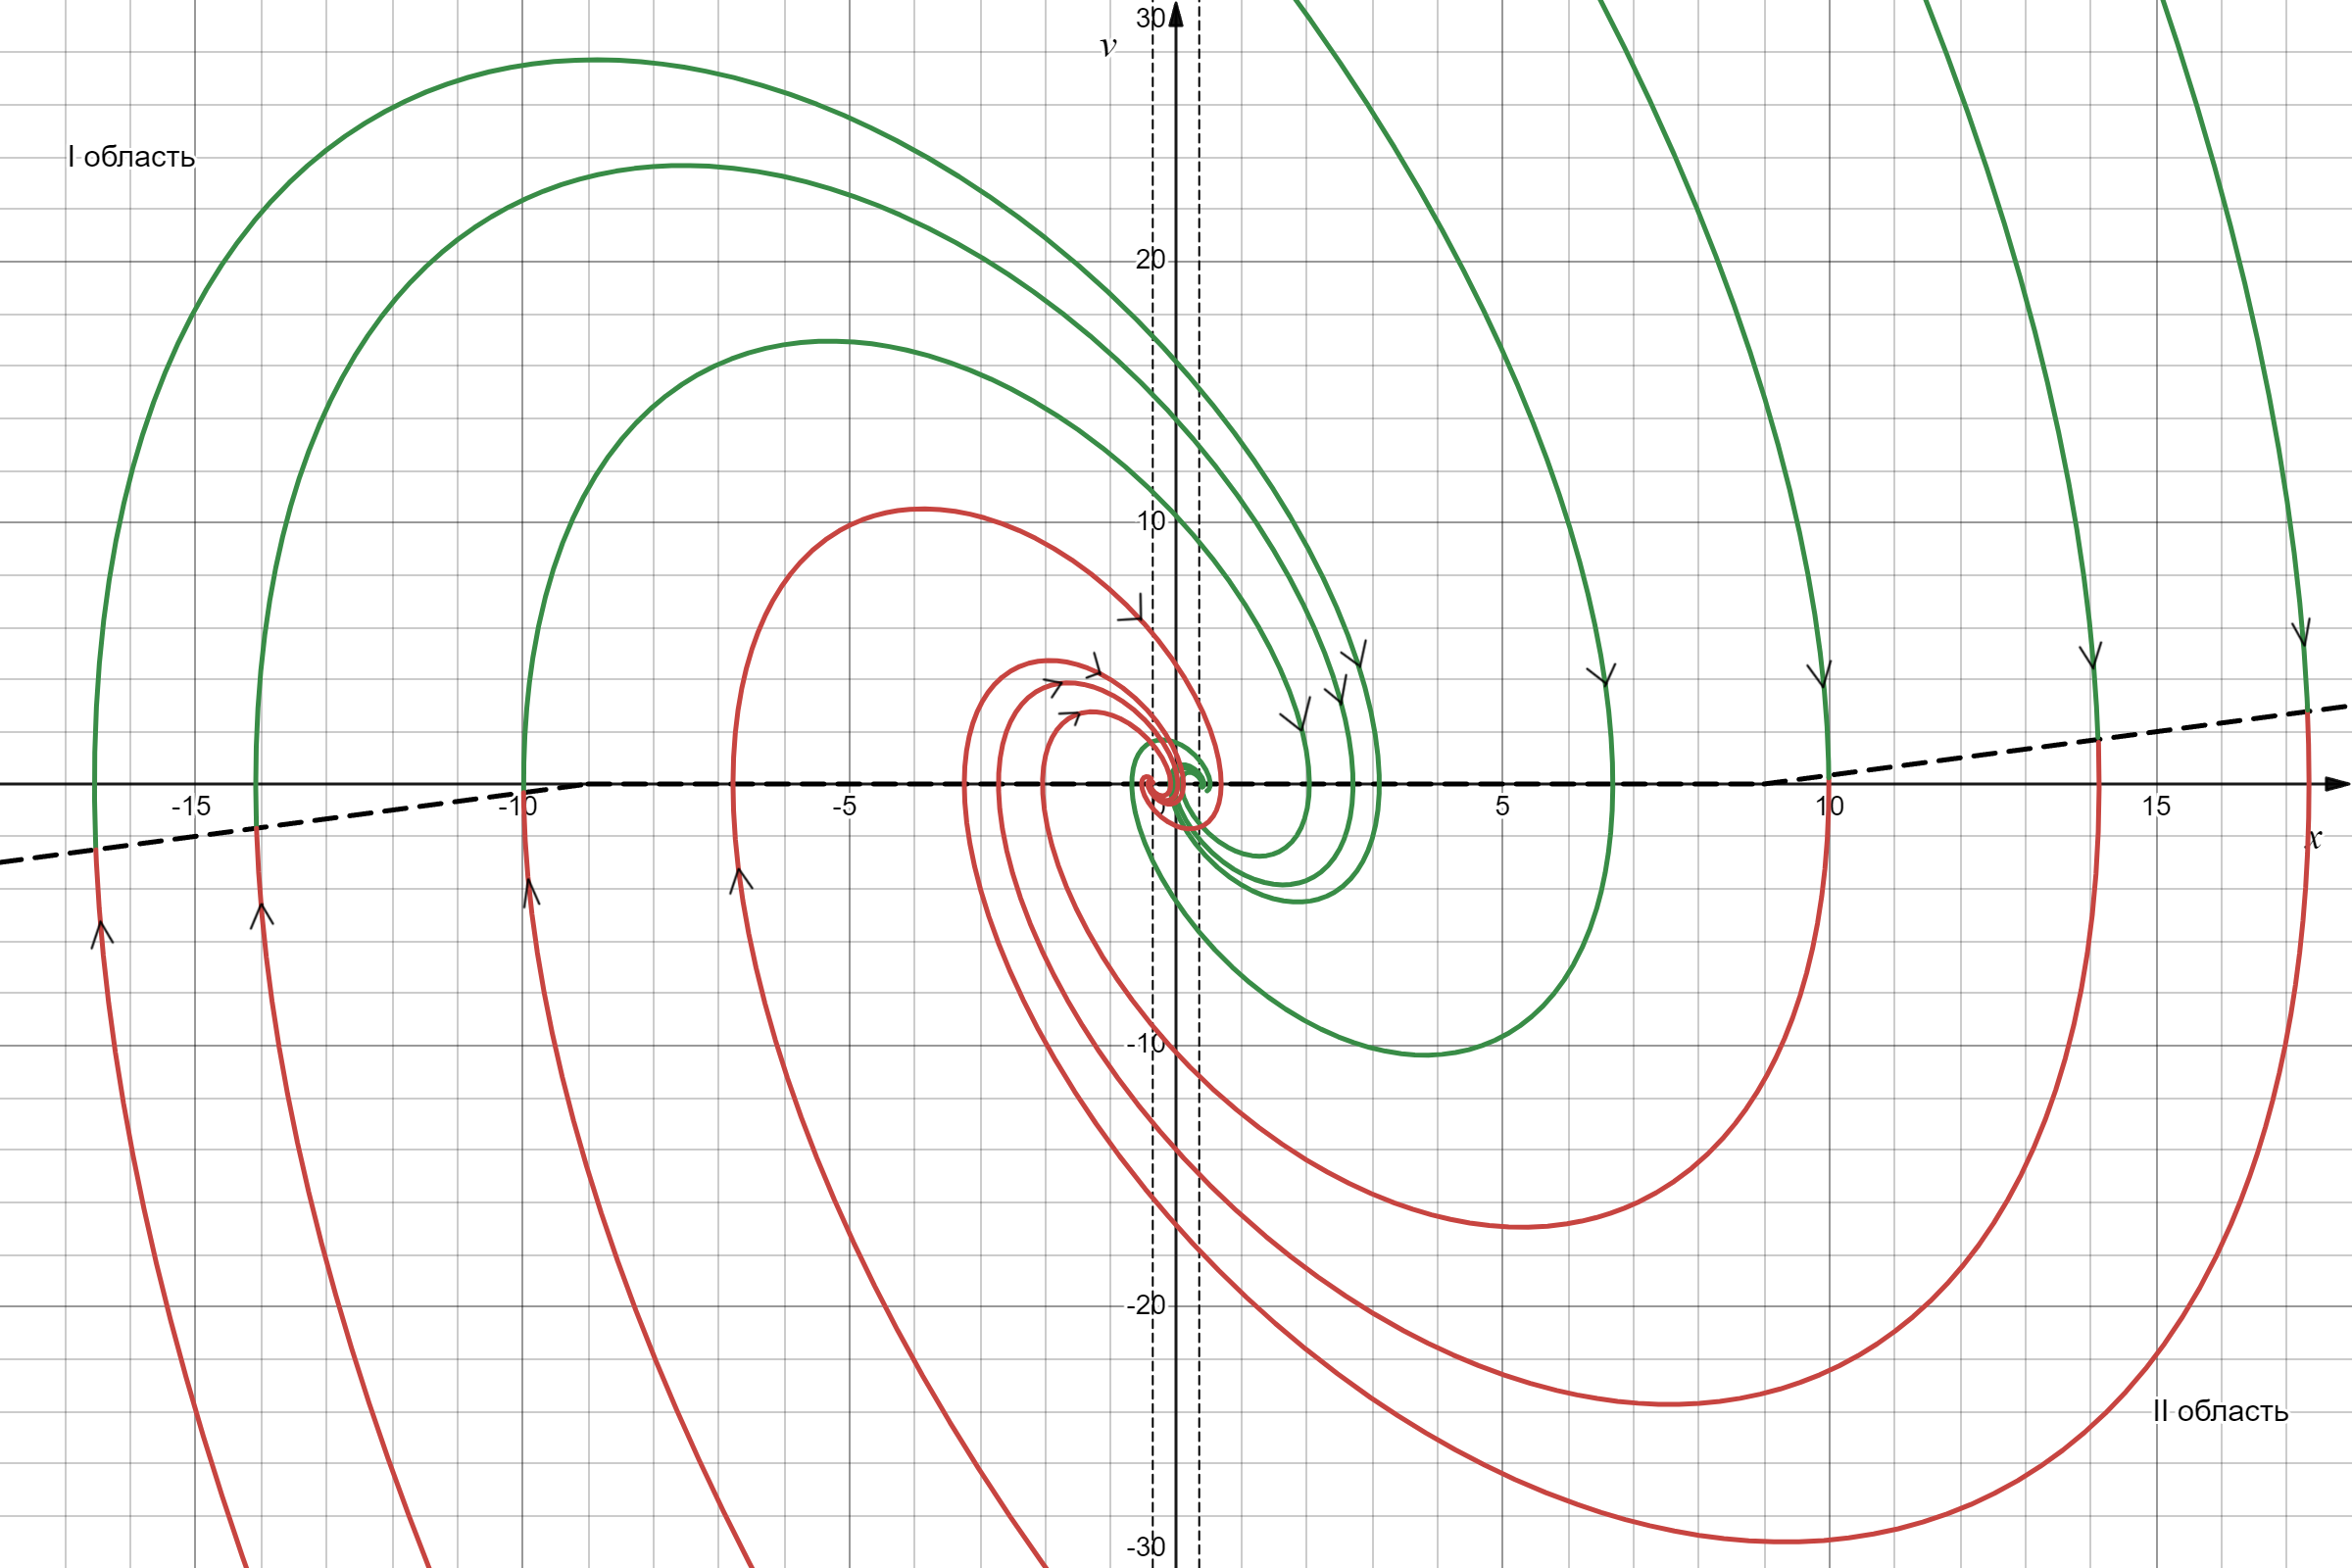
\includegraphics[width=\textwidth]{png/ФП_системы.png}
		\caption{Фазовый портрет исследуемой системы}
		\label{FP}
	\end{figure}
	
	
	По фазовому портрету видно, что особые точки в системе являются асимптотически устойчивыми.
	
	\subsection[Компьютерное моделирование]{Компьютерное моделирование в SimInTech}
	
	Схема для моделирования нелинейной системы автоматического управления (НСАУ) представлена на рис. \ref{s_scheme}. Заданные параметры элементов указаны на рис. \ref{s_params}.
	
	
	\begin{figure}[h]
		\centering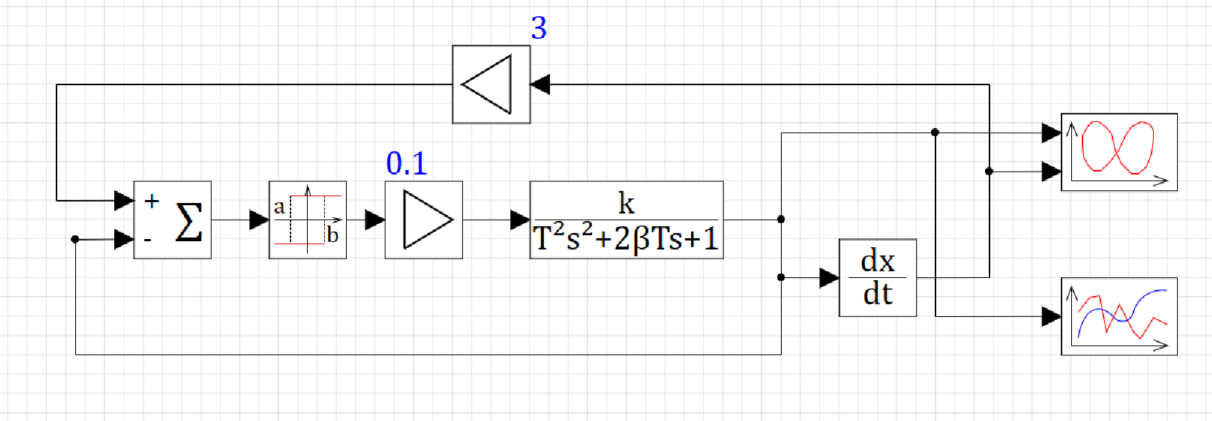
\includegraphics[width=.7\textwidth]{png/Схема_simintech.png}
		\caption{Схема для моделирования НСАУ}
		\label{s_scheme}
	\end{figure}
	
	\noindent{\begin{minipage}{.5\textwidth}
			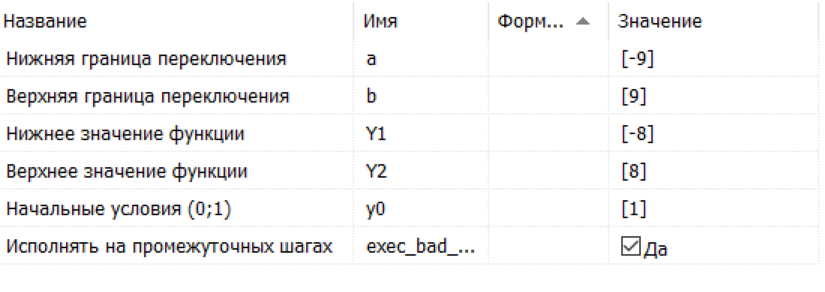
\includegraphics[width=.98\textwidth]{png/Параметры_реле.png}
			\centering а)
		\end{minipage}
		\begin{minipage}{.5\textwidth}
			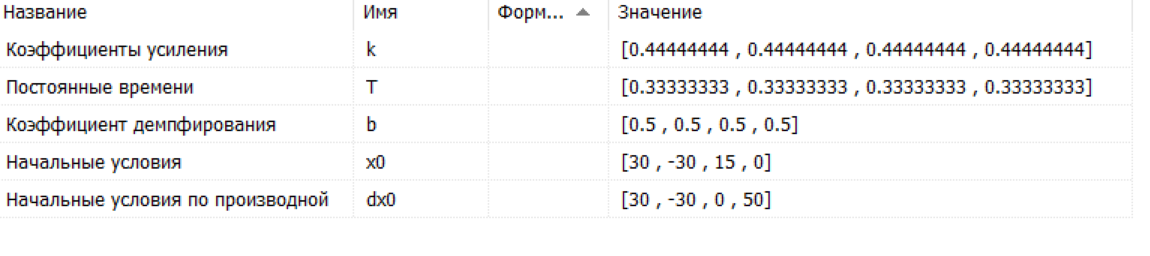
\includegraphics[width=.98\textwidth]{png/Параметры_звено.png}
			\centering б)
		\end{minipage}
		\captionof{figure}{Параметры элементов схемы: а) Двухпозиционное реле с гистерезисом, б) Колебательное звено}
	\label{s_params}}
	
	После расчёта получаем следующие фазовые траектории и вид переходных процессов: рис. \ref{s_FP}, \ref{s_PP}.
	
	\begin{figure}[h]
		\centering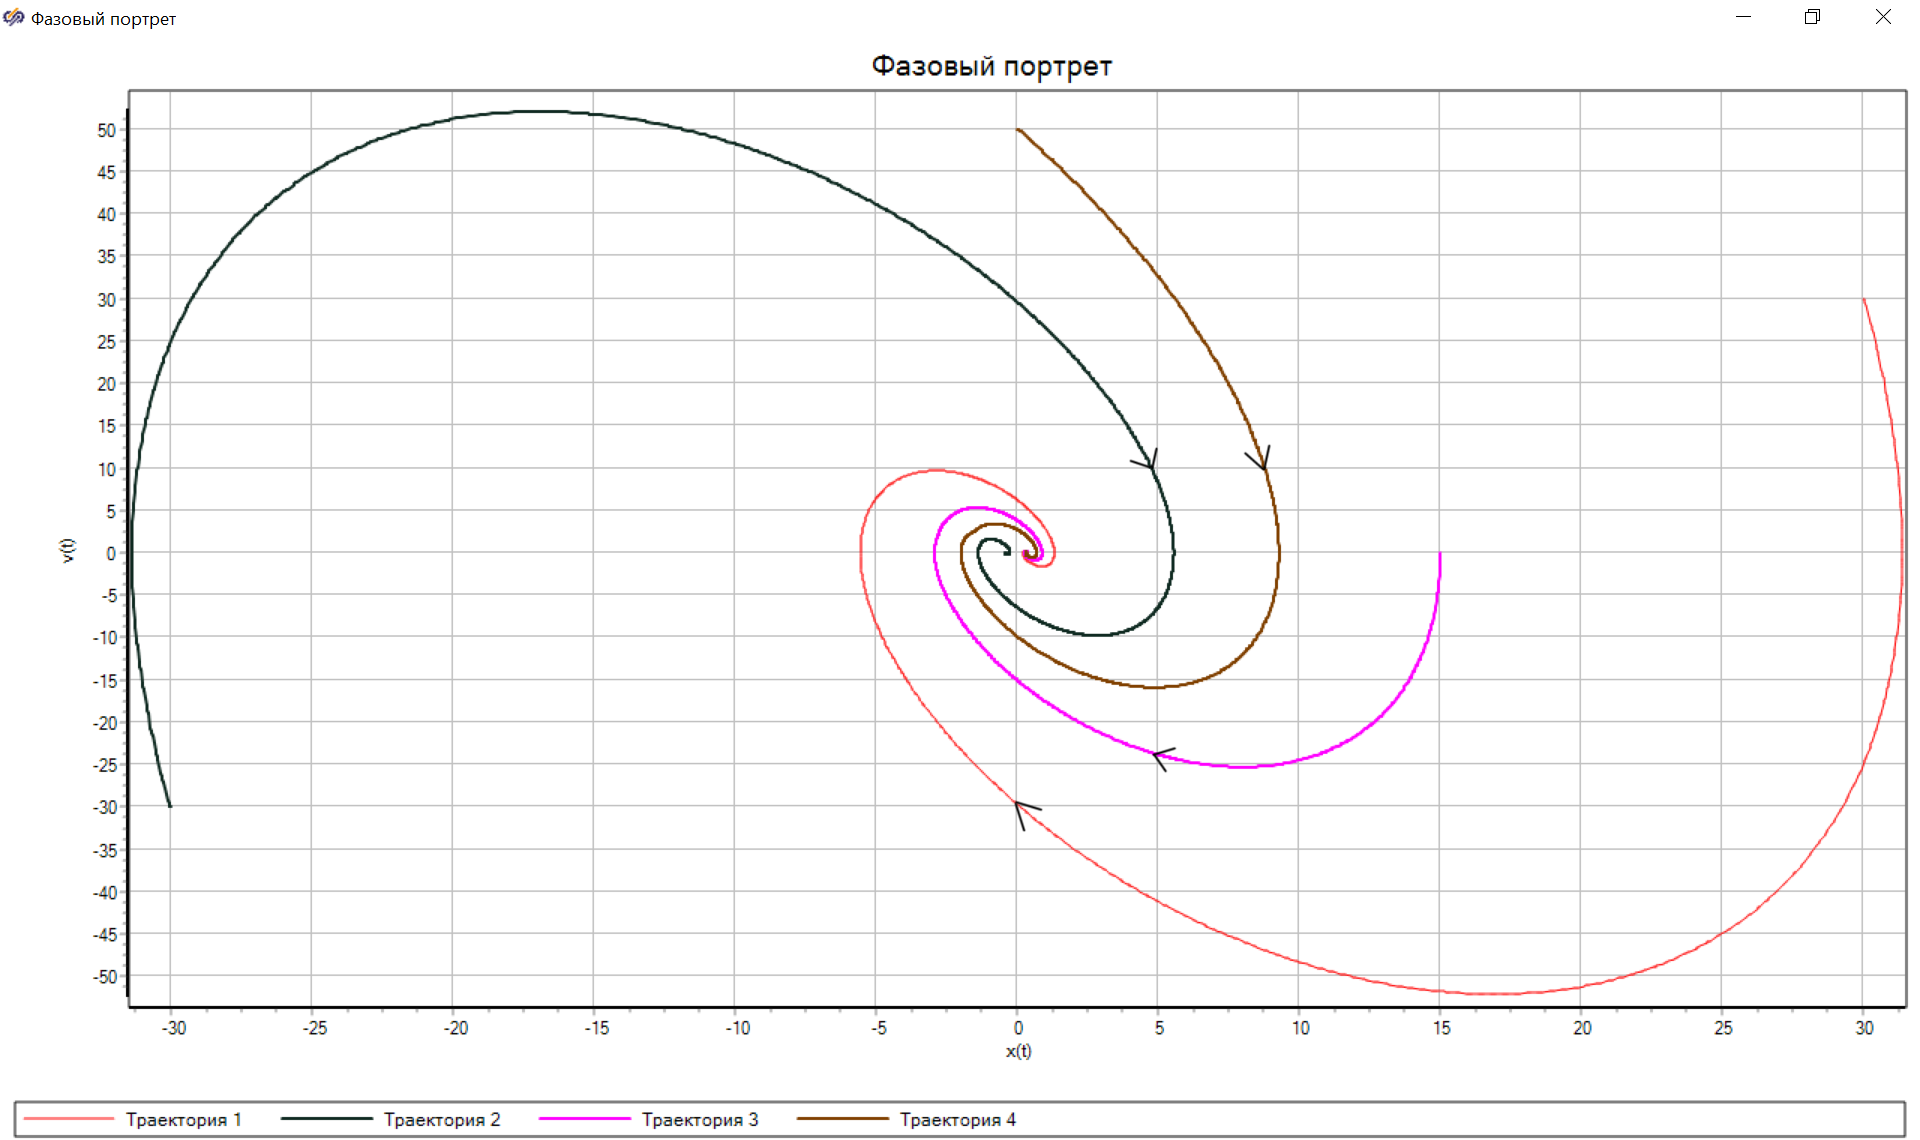
\includegraphics[width=.8\textwidth]{png/ФП_simintech.png}	
		\caption{Фазовый портрет системы}
		\label{s_FP}
	\end{figure}
	
	\begin{figure}[h]
		\centering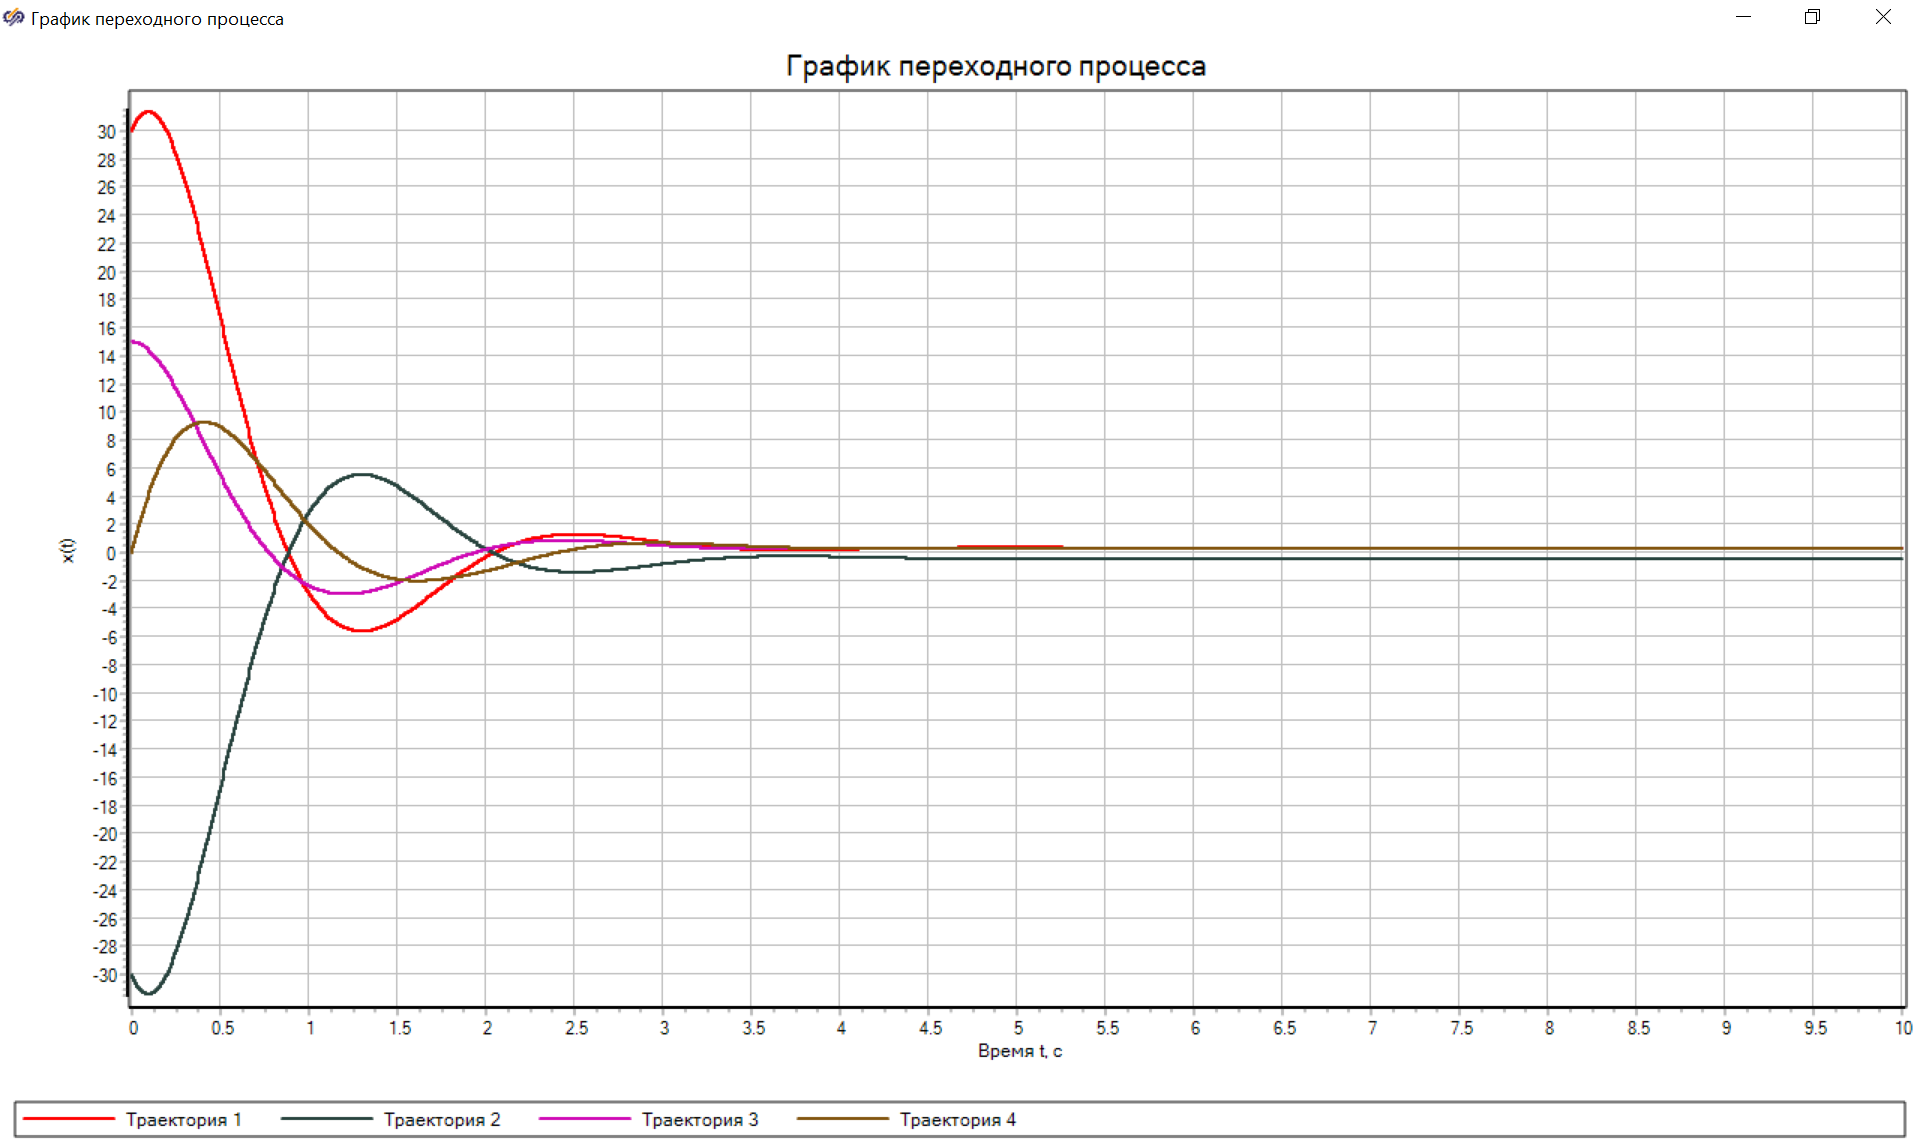
\includegraphics[width=.7\textwidth]{png/ПП_simintech.png}	
		\caption{Переходные процессы в системе}
		\label{s_PP}
	\end{figure}
	
	Получили фазовый портрет такого же вида, что и аналитическим подходом. Особые точки, тоже совпали и имеют координаты $(-0,35,\;0)$ и $(0,35,\,0)$. Переходные процессы получились вида $Ae^{-kt}\sin{(\omega t + \theta)}$.
	
	\subsection[Ширина петли гистерезиса и автоколебания]{Исследование влияния ширины петли гистерезиса на автоколебания}
	
	Будет исследоваться аналогичная НСАУ, но с другим НЭ: трёхпозиционным реле с гистерезисом (рис. \ref{NE2}). Выбрано начальное значение $h=10$.
	
	\begin{figure}[h]
		\centering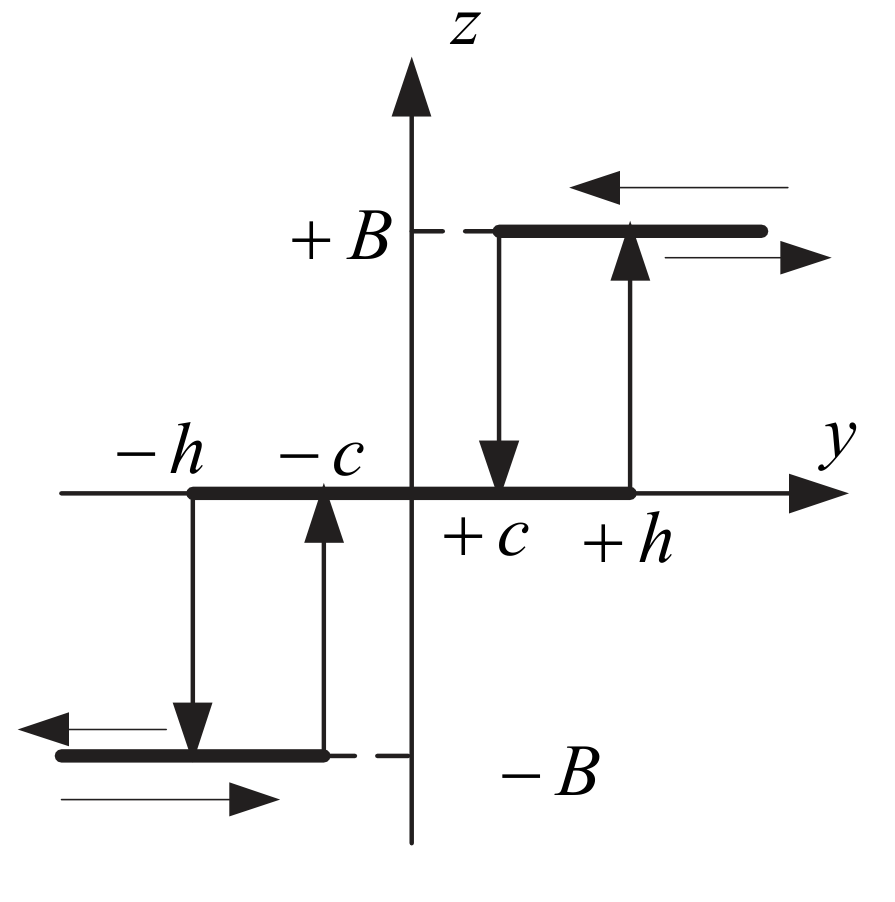
\includegraphics[width=.45\textwidth]{png/НЭ2.png}
		\caption{Характеристика трёхпозиционного реле с гистерезисом}
		\label{NE2}
	\end{figure}
	
	При этих параметрах в системе автоколебаний не наблюдается: рис. \ref{s_lambda1}
	
	\begin{figure}[h]
		\centering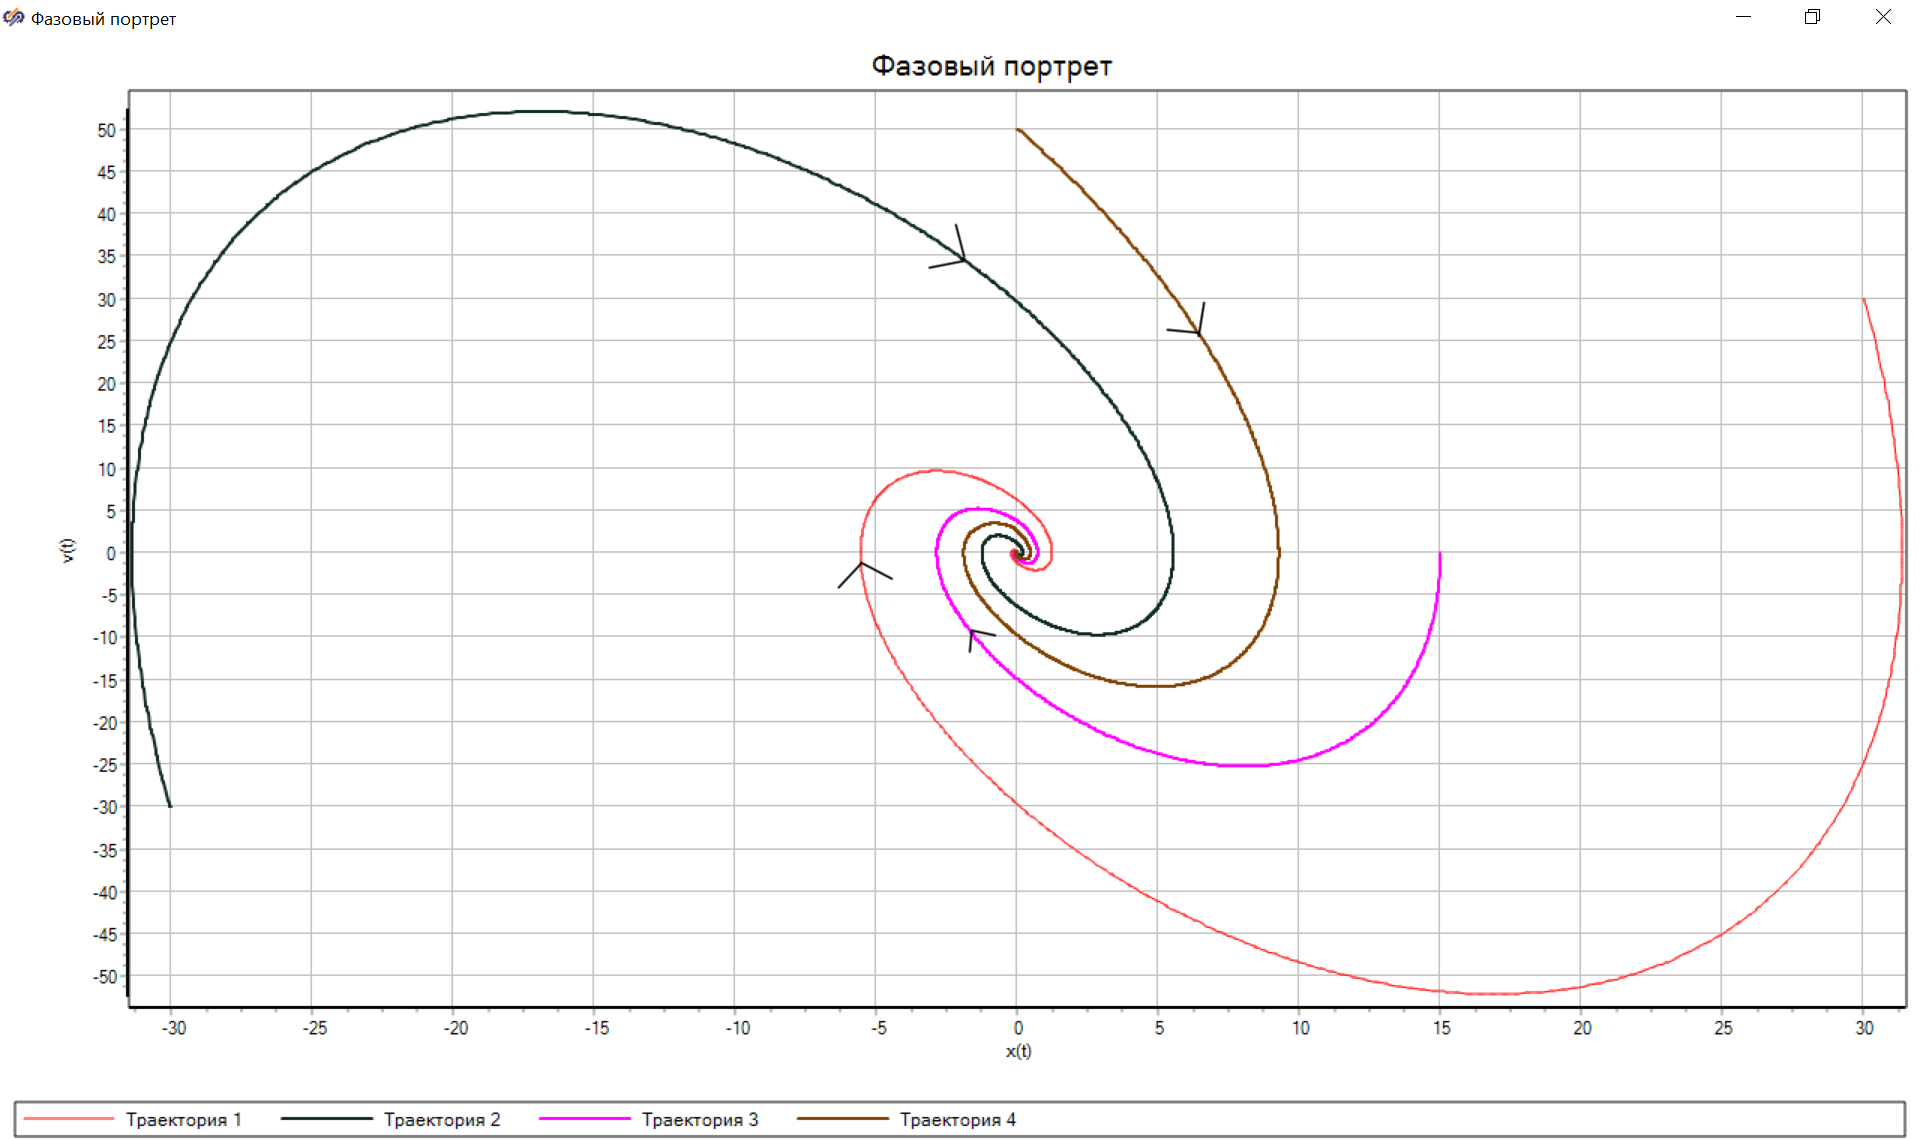
\includegraphics[width=.7\textwidth]{png/FP_lambda1.png}
		\caption{Фазовый портрет при изначальных параметрах}
		\label{s_lambda1}
	\end{figure}
	
	Зафиксируем значение $c=9$ и увеличим дальнюю от нуля границу переключения реле: $h=15$. Это действие никак не повлияло на возникновение автоколебаний в системе (рис. \ref{s_lambda2}).
	
	\begin{figure}[h]
		\centering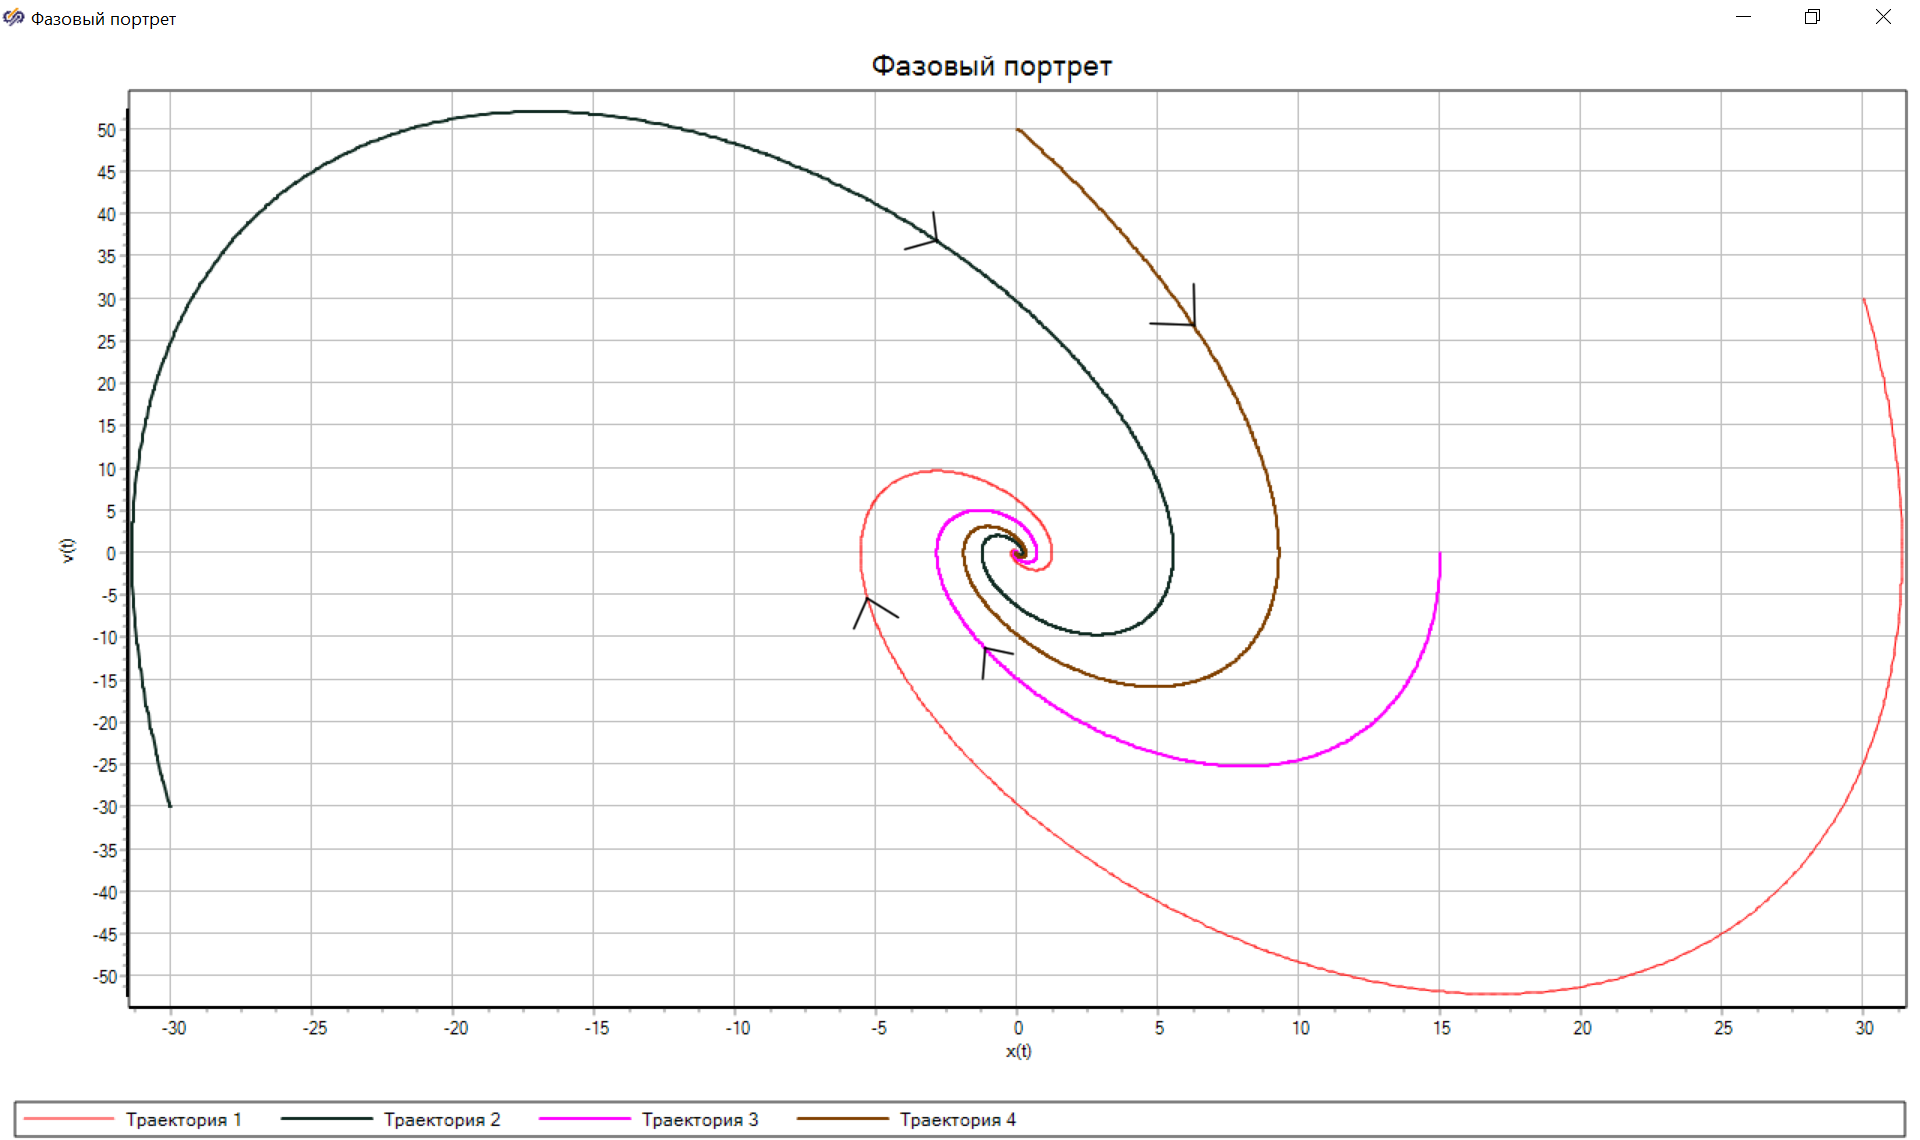
\includegraphics[width=.7\textwidth]{png/FP_lambda2.png}
		\caption{Фазовый портрет при $c=9$ и $h=15$}
		\label{s_lambda2}
	\end{figure}
	
	Зафиксируем значение $h=10$ и увеличим ближнюю к нулю границу переключения реле: $c=0.1$. Это действие никак не повлияло на возникновение автоколебаний в системе (рис. \ref{s_lambda3}).
	
	\begin{figure}[h]
		\centering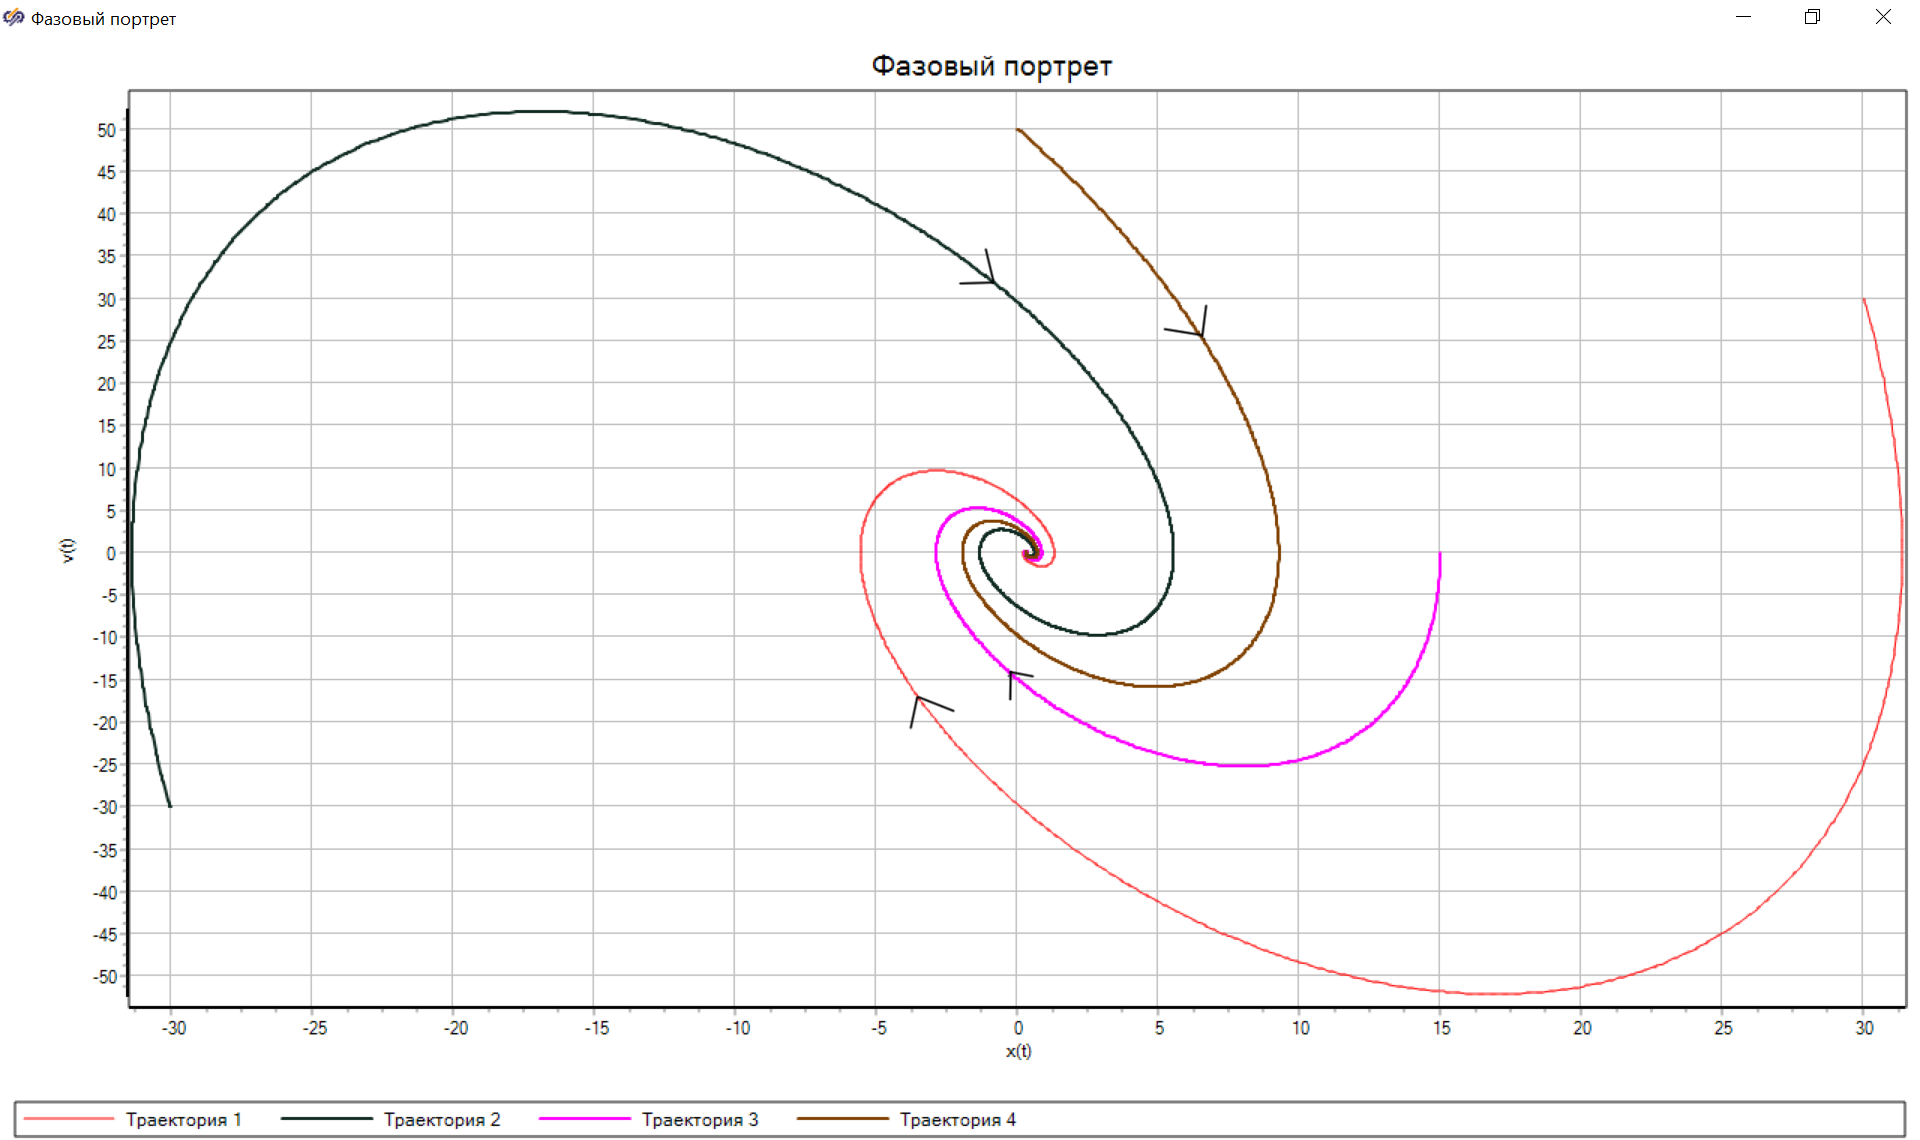
\includegraphics[width=.7\textwidth]{png/FP_lambda3.png}
		\caption{Фазовый портрет при $c=0.1$ и $h=10$}
		\label{s_lambda3}
	\end{figure}
	
	Таких результатов можно ожидать, поскольку как видно из рис. \ref{FP} траектории всех типов около полупрямых переключения явно идут в одном <<закручивающемся>> направлении. Различия между траекториями разных типов начинают проявляться вблизи особых точек, поэтому для возникновения автоколебаний переключение должно происходить именно там.
	
	С учётом того, что НЭ является трёхпозиционным реле с пассивным гистерезисом, автоколебания возникнут при одновременном уменьшении $c$ и $h$.
	
	Одновременное уменьшение этих параметров будет соответствовать уменьшению зоны нечувствительности, а не ширины петли гистерезиса. Поэтому делаем следующий вывод: для данной системы с трёхпозиционным реле с гистерезисом при начальных параметрах $c_0 = 9,\;h_0=10$ изменение ширины петли гистерезиса никак не влияет на появление автоколебаний.
	
	Тогда отсутствует граничная ширина гистерезиса, при которой появляются автоколебания. 
	
	Сузим зону нечувствительности для дальнейших исследований: для трёхпозиционного реле без гистерезиса наблюдаются автоколебания при $c=1.5$ -- выберем это значение для наших исследований, и найдём максимальную ширину петли гистерезиса, при которой автоколебания наблюдаются.
	
	Автоколебания присутствуют в системе при $c\leq h \leq 2.1$ рис. \ref{s_lambda4}
	
	\noindent{\begin{minipage}{.5\textwidth}
			\centering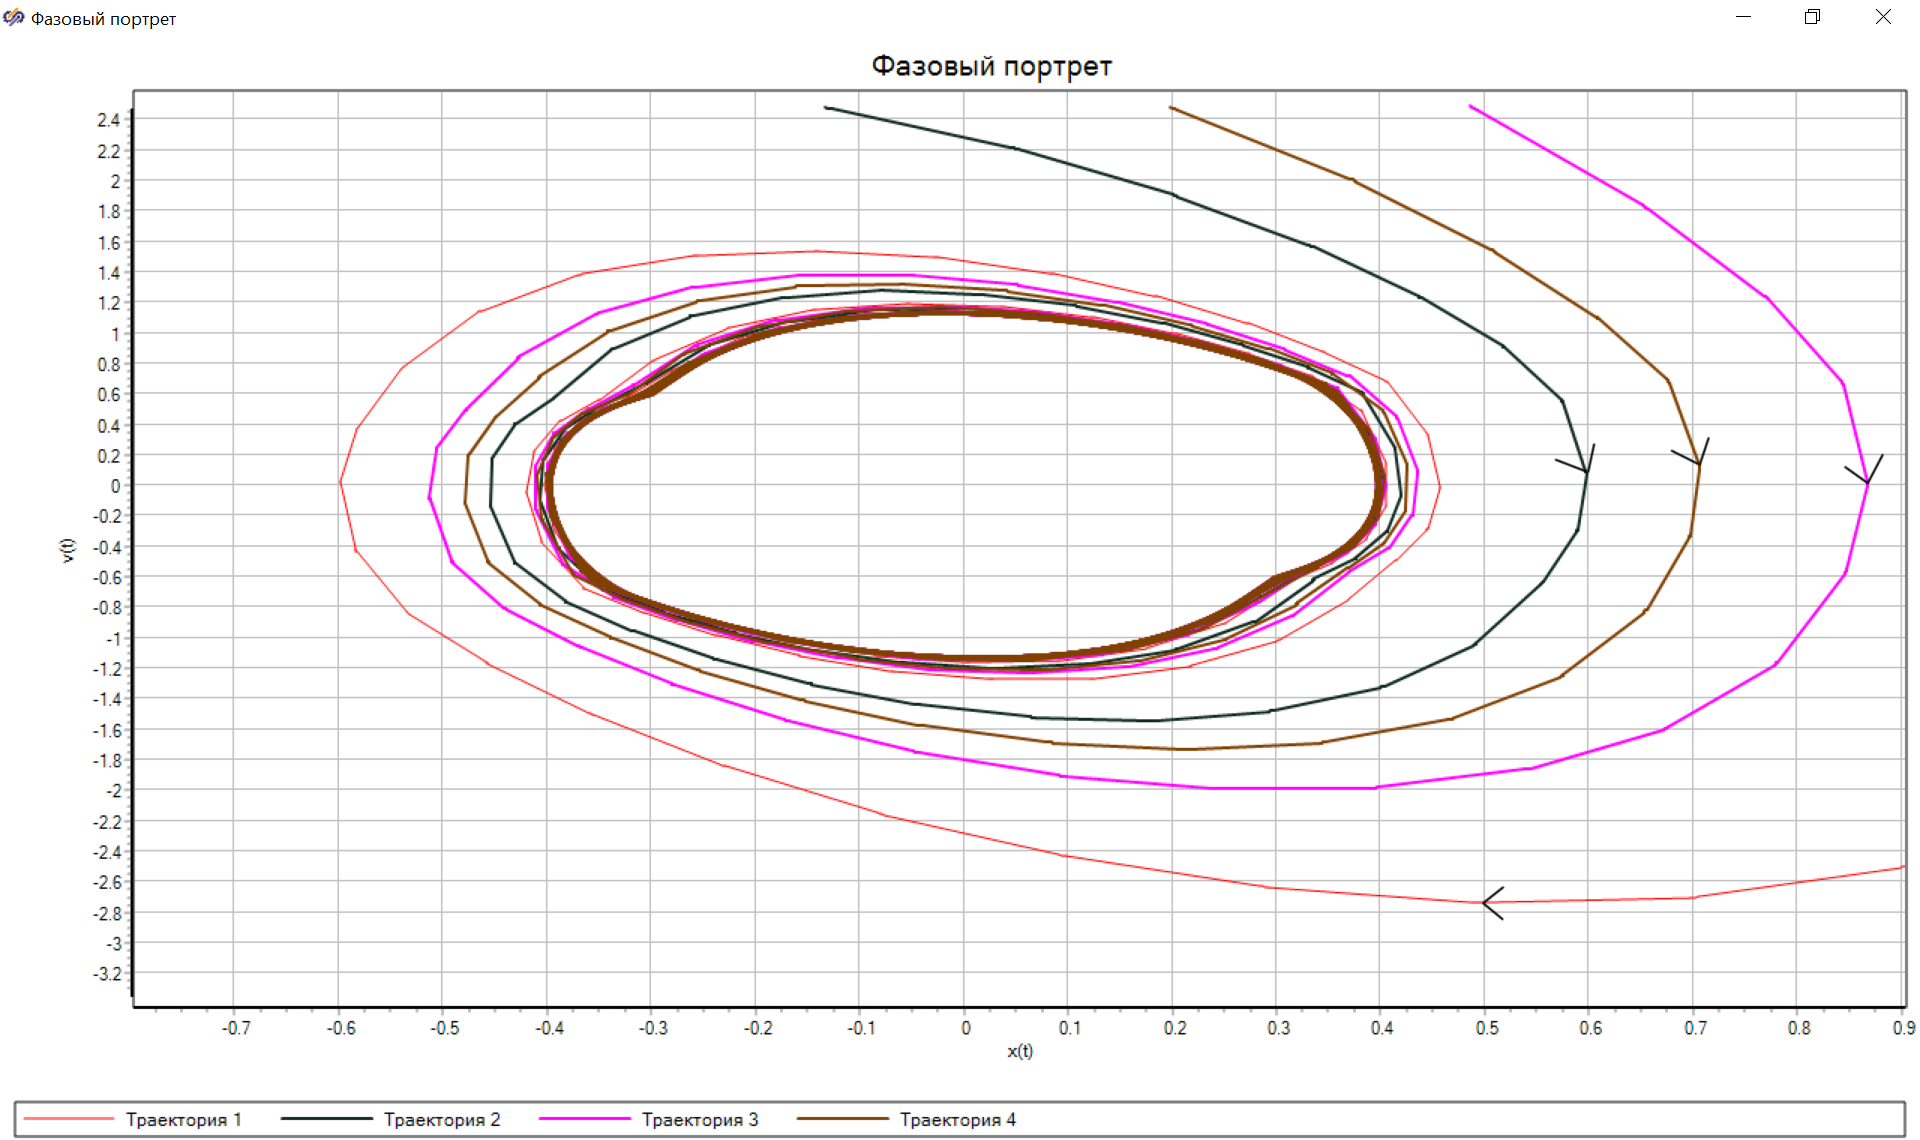
\includegraphics[width=\textwidth]{png/FP_lambda4.png}	
		\end{minipage}
		\begin{minipage}{.5\textwidth}			\centering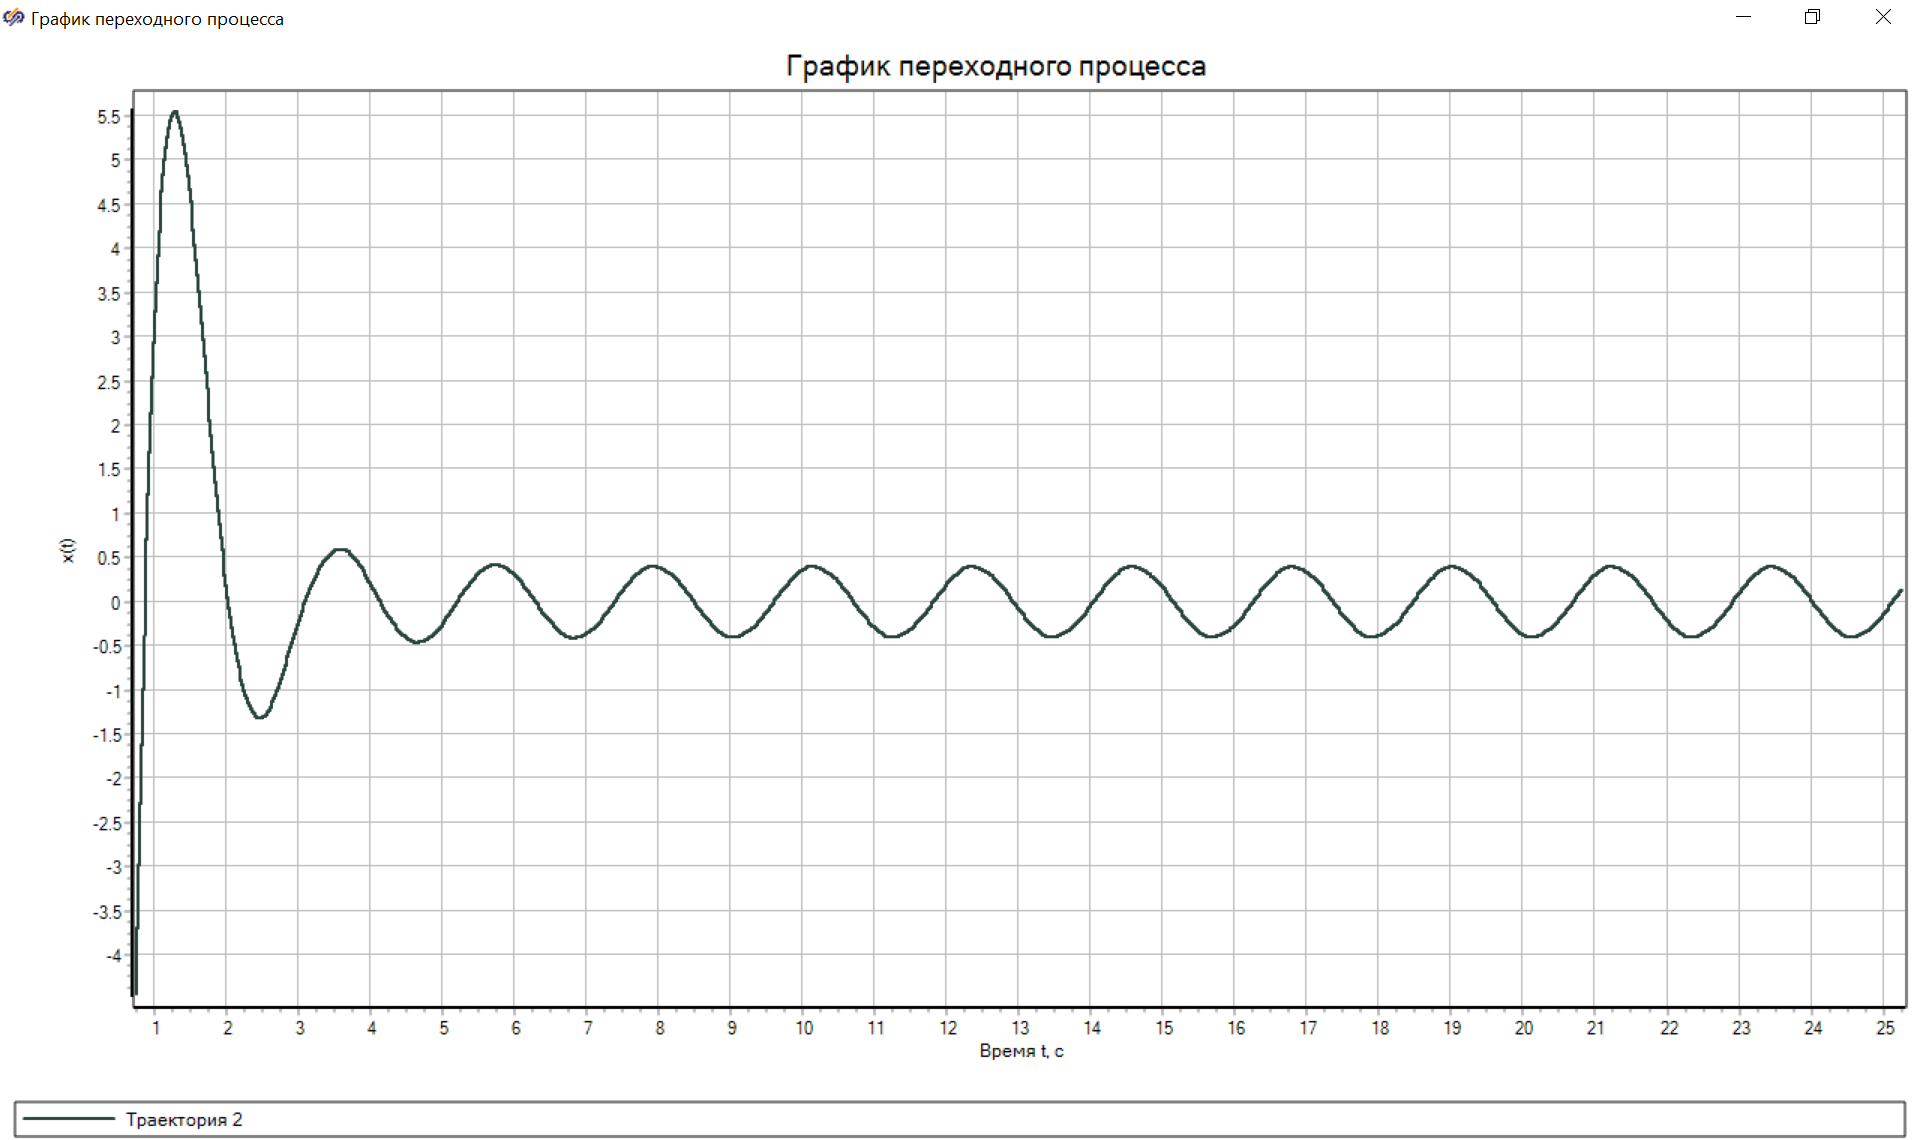
\includegraphics[width=\textwidth]{png/PP_lambda4.png}		
		\end{minipage}
		\captionof{figure}{Автоколебания при $c=1.5$ и $h=2.1$}
		\label{s_lambda4}
	}
	
	При большей ширине автоколебаний нет: рис. \ref{s_lambda5}. Тогда получаем следующую максимальную ширину петли гистерезиса, при которой наблюдаются автоколебания:
	\begin{equation*}
		\lambda_{\max} = \frac{h_{\max}-c}{h_{\max}} = \frac{2.1-1.5}{2.1} = 0.29
	\end{equation*}
	
	При этом амплитуда автоколебаний $A_m = 0.406$ и период $T = 2.3$ с.
	
	
	\begin{figure}[h]
		\centering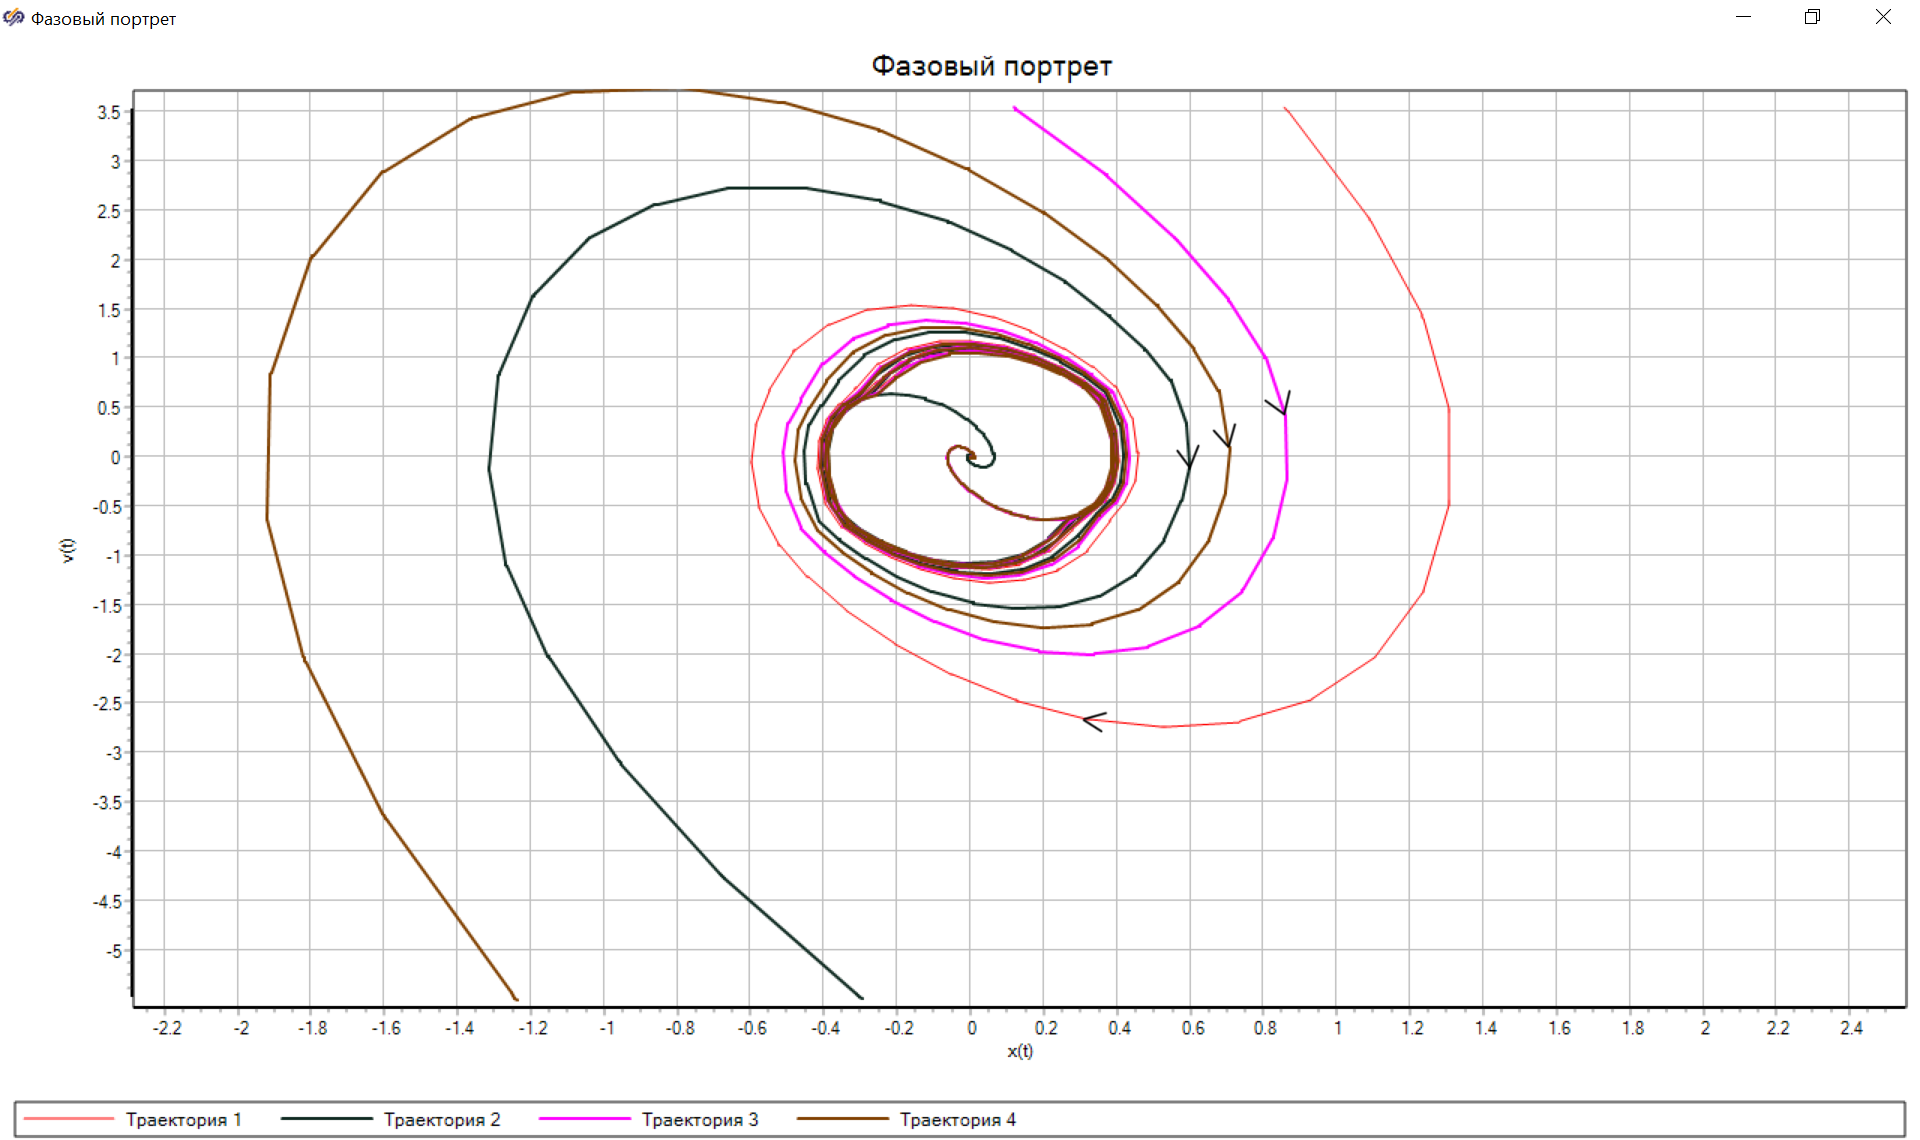
\includegraphics[width=.5\textwidth]{png/FP_lambda5.png}
		\caption{Фазовый портрет при $c=1.5$ и $h=2.15$}
		\label{s_lambda5}
	\end{figure}
	
	\subsection[Автоколебания при большем КУ регулятора]{Исследование автоколебаний при большем коэффициенте усиления регулятора}
	
	Увеличим $W_1(p)$ в пять раз: $W_1(p) = 5\cdot0.1 = 0.5$. Тогда при $c=1.5,\, h=2.1$ получаем следующие автоколебания: рис. \ref{s_lambda6}
	
	\begin{figure}[h]
		\centering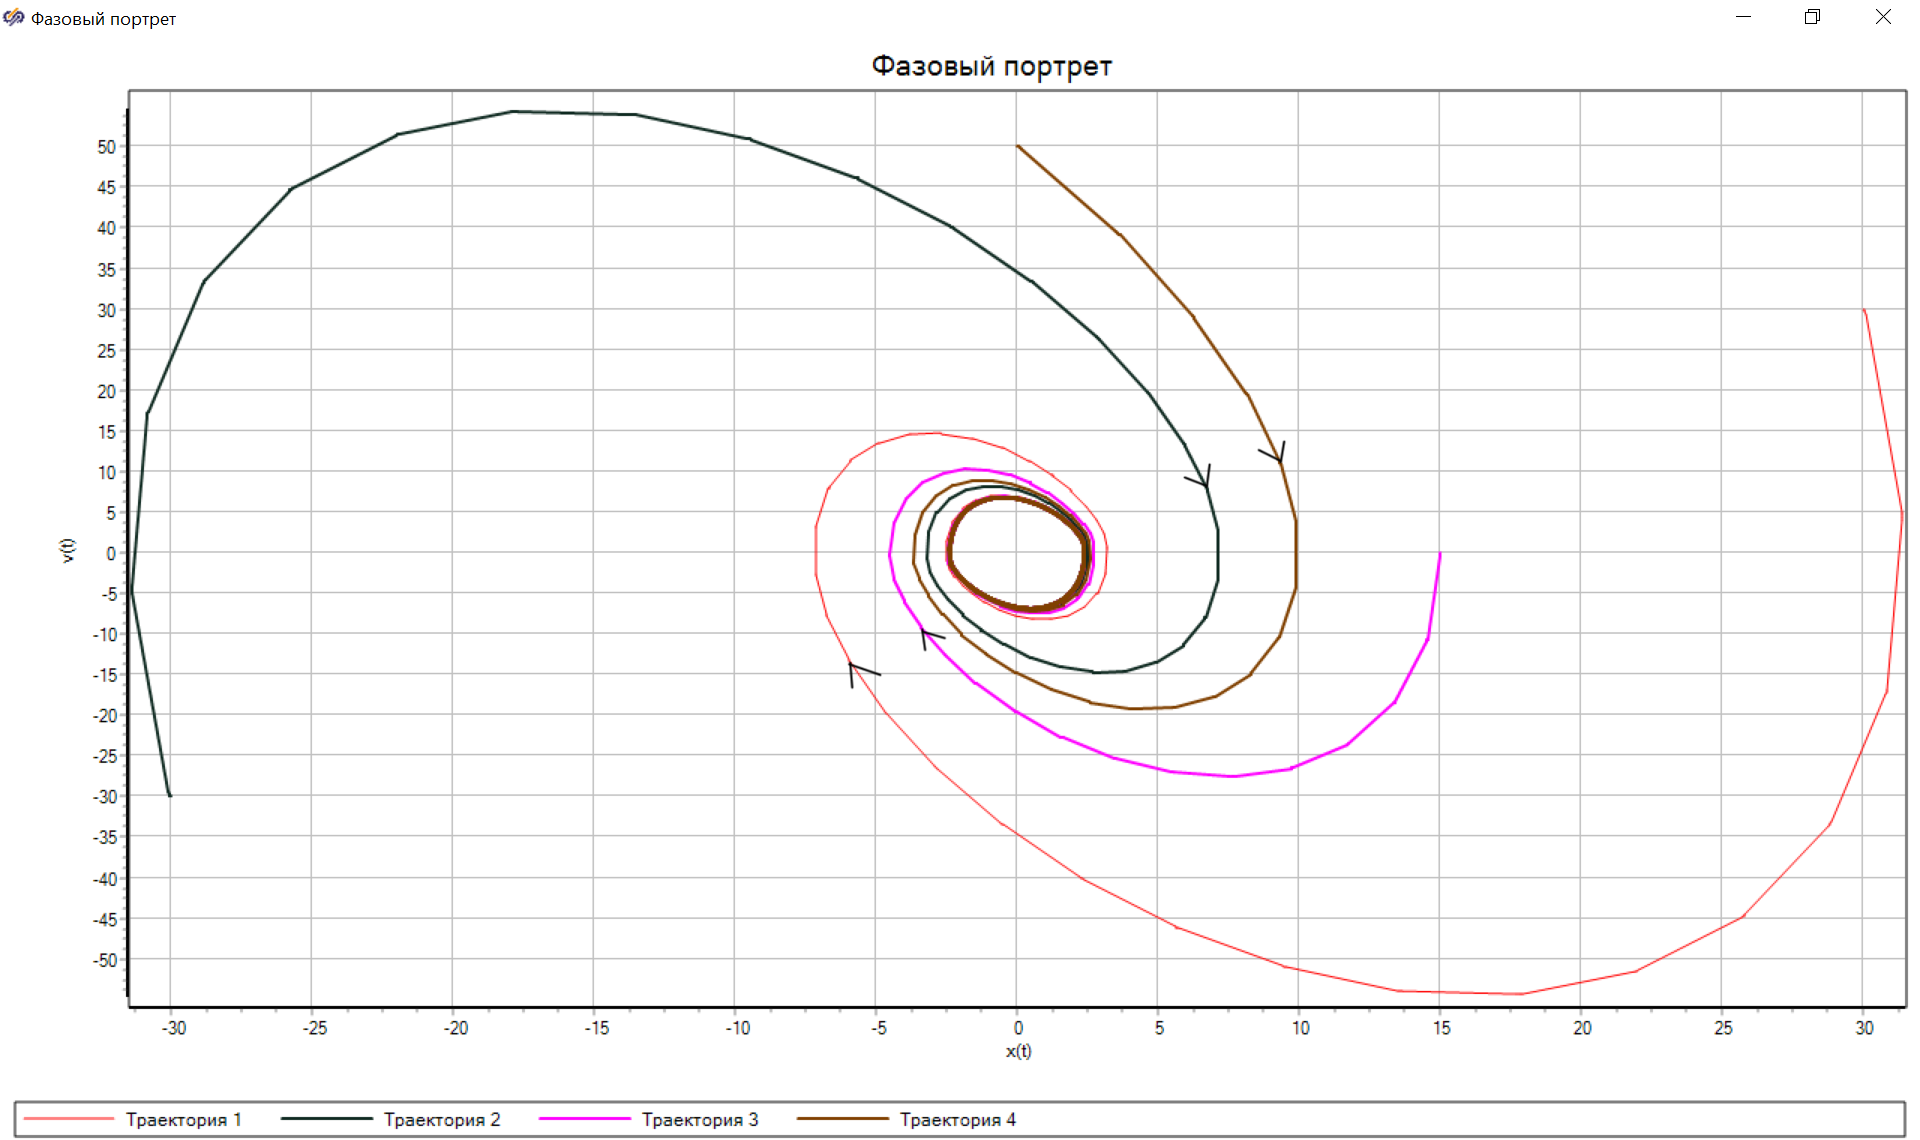
\includegraphics[width=.7\textwidth]{png/FP_lambda6.png}
		\caption{Автоколебания при $c=1.5$, $h=2.15$ и увеличенном КУ регулятора}
		\label{s_lambda6}
	\end{figure}
	
	\begin{figure}[h]
		\centering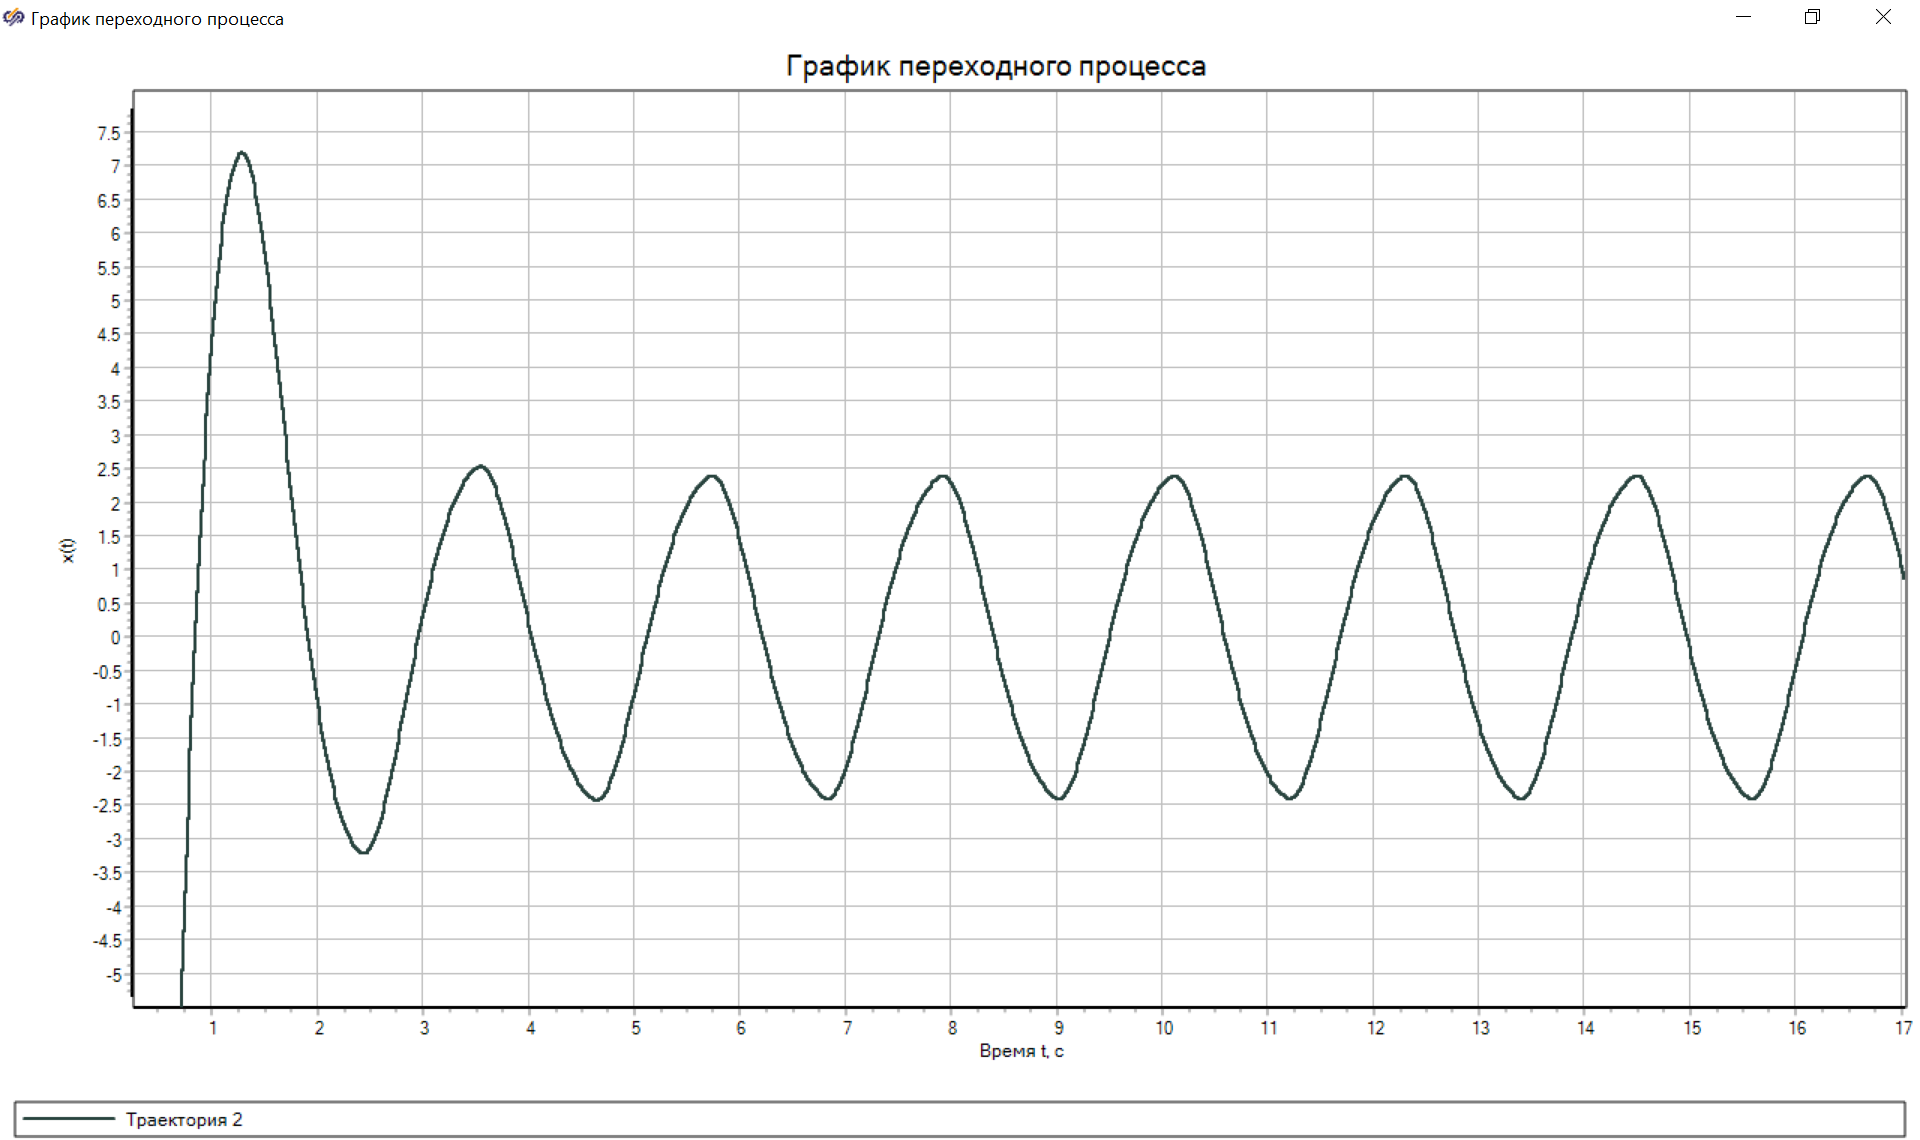
\includegraphics[width=.7\textwidth]{png/PP_lambda6.png}
		\caption{Переходной процесс при $c=1.5$, $h=2.15$ и увеличенном КУ регулятора}
		\label{sp_lambda6}
	\end{figure}
	
	Параметры автоколебаний: амплитуда $A_m = 2.41$, период $T=2.2$ с.
	
	\section[Метод Гольдфарба]{Исследование параметров автоколебаний методом Гольдфарба}
	
	\subsection{Исходная система}
	
	Приведём систему рис. \ref{scheme} к виду модели Гаммерштейна: рис. \ref{scheme2}
	
	\begin{figure}[h]
		\centering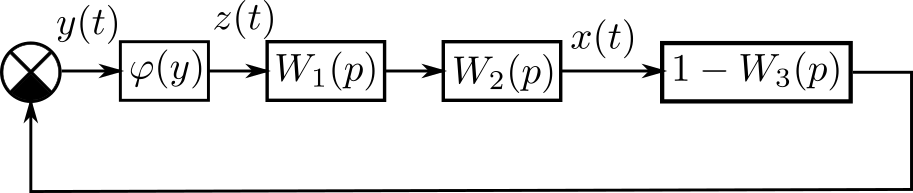
\includegraphics[width=.7\textwidth]{png/Схема_Гаммерштейн.png}
		\caption{Схема в виде модели Гаммерштейна}
		\label{scheme2}
	\end{figure}
	
	Полученная система состоит из НЭ $\varphi(y)$ и линейной части  с передаточной функцией:
	\begin{equation*}
		W_{\text{лч}}(p) = W_1(p)W_2(p)(1-W_3(p)) = 0.1\cdot\frac{4}{p^2+3p+9}\cdot(1-3p)
	\end{equation*} 
	
	В соответствии с методом Гольдфарба наличие автоколебаний соответствует решению уравнения:
	\begin{equation*}
		W_{\text{лч}}(j\omega) = -z(A),\;z(A) = \frac{1}{W_{\text{нэ}}(A)}
	\end{equation*}
	\begin{equation*}
		W_\text{нэ} = a(A) + jb(A),\; a,\,b\text{ -- коэффициенты гармонической линеаризации}
	\end{equation*}
	
	Эти коэффициенты известны для данного типа НЭ и равны:
	\begin{equation*}
		a(A) = \frac{2B}{\pi A^2}(\sqrt{A^2 - h^2} + \sqrt{A^2 - c^2}) = \frac{16}{\pi A^2}(\sqrt{A^2 - 100} + \sqrt{A^2 - 81})
	\end{equation*}
	\begin{equation*}
		b(A) = -\frac{2B(h-c)}{\pi A^2} = -\frac{16}{\pi A^2}
	\end{equation*}
	
	Построим АФХ линейной части и $-z(A)$ на комплексной плоскости: рис. \ref{GF1}. Как видим, данное уравнение не имеет решений, поэтому такая система не имеет автоколебаний.
	
	\begin{figure}[h]
		\centering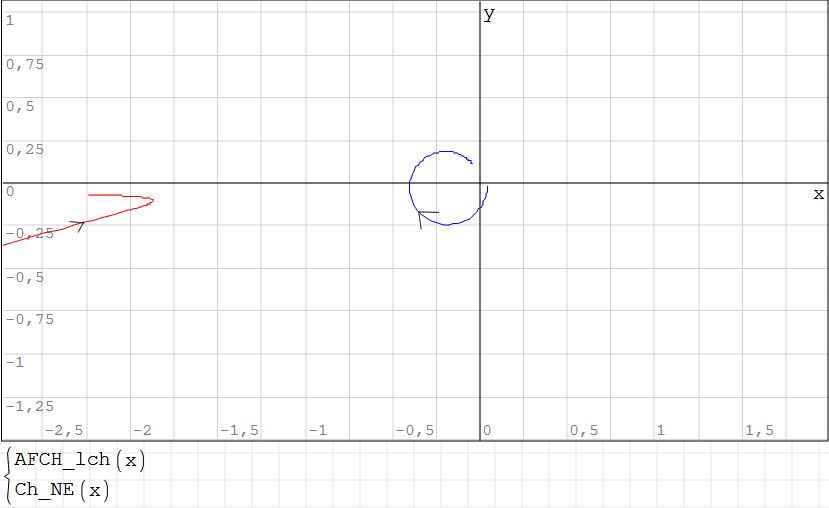
\includegraphics[width=.7\textwidth]{png/GF1.png}
		\caption{Нахождение автоколебаний для $c=9$, $h=10$}
		\label{GF1}
	\end{figure}
	
	\subsection{Система с $\lambda_{\max}$}
	
	Исследуем таким же образом систему, в которой параметры НЭ: $c=1.5$, $h=2.1$. В ней коэффициенты гармонической линеаризации равны:
	\begin{equation*}
		a(A) = \frac{16}{\pi A^2}(\sqrt{A^2 - 2.1^2} + \sqrt{A^2 - 1.5^2})
	\end{equation*}
	\begin{equation*}
		b(A) = -\frac{16\cdot 0.6}{\pi A^2} = -\frac{9.6}{\pi A^2}
	\end{equation*}
	
	Получаем следующее графическое представление инверсной характеристики: рис. \ref{GF2}. Получили два решения:
	\begin{itemize}
		\item Неустойчивые автоколебания при $A_{y_m} = 2.22$ и $\omega = 2.8\Rightarrow T=2,24$;
		\item Устойчивые автоколебания при $A_{y_m} = 3.5$ и $\omega = 3.01\Rightarrow T=2,09$.
	\end{itemize}
	
	Найдём амплитуду устойчивых автоколебаний $x(t)$:
	\begin{equation*}
		A_m = \frac{A_{y_m}}{|1-W_3(p)|} = \frac{A_{y_m}}{\sqrt{1+(3\omega)^2}} = \frac{3.5}{\sqrt{1+(3\cdot3.01)^2}} = 0.39
	\end{equation*}
	
	\begin{figure}[h]
		\centering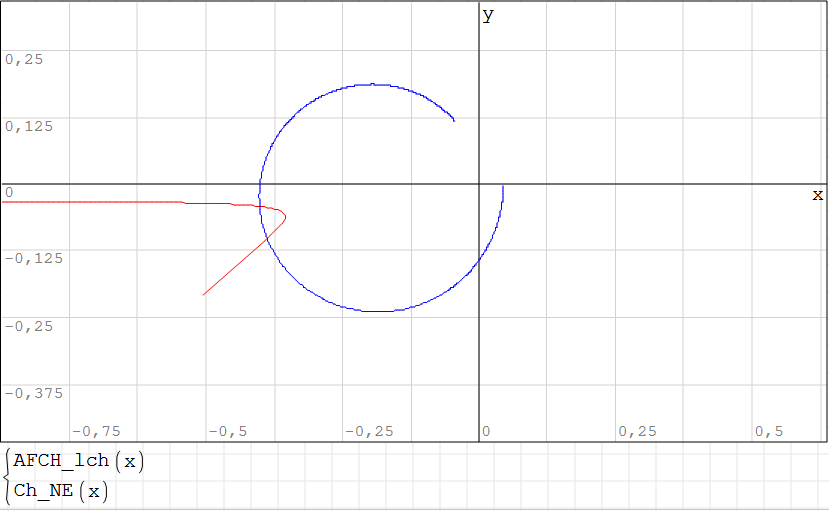
\includegraphics[width=.7\textwidth]{png/GF2.png}
		\caption{Нахождение автоколебаний для $c=1.5$, $h=2.1$}
		\label{GF2}
	\end{figure}
	
	\subsection{Система с увеличенным КУ регулятора}
	
	Теперь исследуем параметры автоколебаний в системе с увеличенным в 5 раз КУ регулятора.
	
	\begin{equation*}
		W_{\text{лч}}(p) = 5\cdot W_1(p)W_2(p)(1-W_3(p)) = 5\cdot0.1\cdot\frac{4}{p^2+3p+9}\cdot(1-3p)
	\end{equation*} 
	\begin{equation*}
		a(A) = \frac{16}{\pi A^2}(\sqrt{A^2 - 2.1^2} + \sqrt{A^2 - 1.5^2})
	\end{equation*}
	\begin{equation*}
		b(A) = -\frac{16\cdot 0.6}{\pi A^2} = -\frac{9.6}{\pi A^2}
	\end{equation*}
	
	Итоговое графическое представления решений уравнения автоколебаний: рис. \ref{GF3}. Получили одно решение соответствующее устойчивым автоколебаниям с $A_{y_m} = 20.3$ и $\omega = 3.15\Rightarrow T=1.99$.
	
	\begin{figure}[h]
		\centering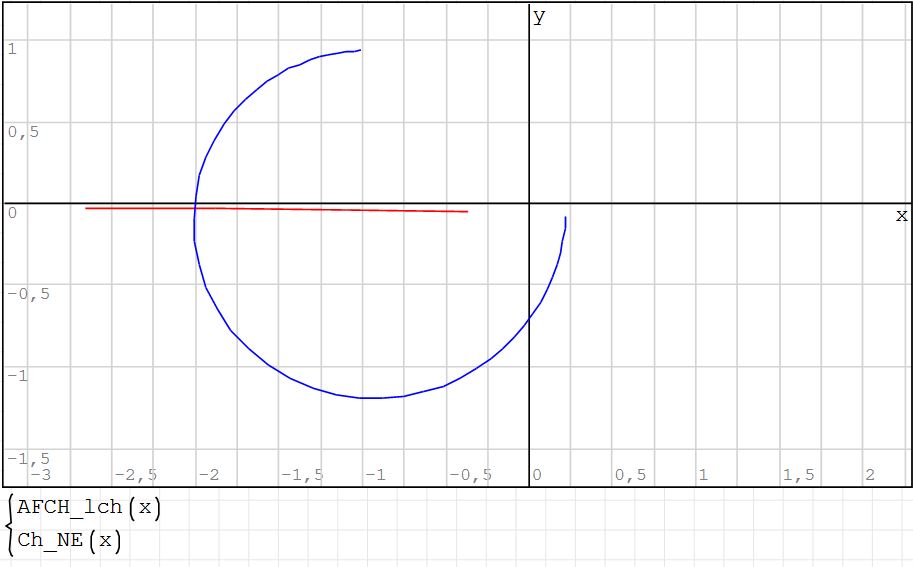
\includegraphics[width=.7\textwidth]{png/GF3.png}
		\caption{Нахождение автоколебаний для $c=1.5$, $h=2.1$ и увеличенного КУ регулятора}
		\label{GF3}
	\end{figure}
	
	Найдём амплитуду устойчивых автоколебаний $x(t)$:
	\begin{equation*}
		A_m = \frac{A_{y_m}}{|1-W_3(p)|} = \frac{A_{y_m}}{\sqrt{1+(3\omega)^2}} = \frac{20.3}{\sqrt{1+(3\cdot3.15)^2}} = 2,14
	\end{equation*}
	
	\section{Сравнение полученных результатов и выводы}
	
	Полученные параметры автоколебаний сведены в таблицу \ref{table_res}. Как видим, результаты, полученные по методу Гольдфарба, отличаются, но не сильно от результатов моделирования. 
	
	Различие обосновывается в нестрогости выполнения предположения метода Гольдфарба: гипотезы фильтра. По предположению линейная часть является идеальным фильтром низких частот (ФНЧ), пропускающим только первую гармонику сигнала. В нашем случае, линейная часть действительно является ФНЧ, но это неидеальный фильтр.
	
	Если численно сравнить пропускную способность линейной части основной гармоники $\omega_0 = 3\,\text{с}^{-1}$ и последующих гармоник, то $\dfrac{|W_\text{лч}(3j)|}{|W_\text{лч}(6j)|} = 1.8,\;\dfrac{|W_\text{лч}(3j)|}{|W_\text{лч}(9j)|} = \\ = 2.9,\,\dots\,,\dfrac{|W_\text{лч}(3j)|}{|W_\text{лч}(3nj)|} \approx n$, то есть, так как уже вторая гармоника пропускается хуже в $1.8>\sqrt{2}$ раз первой, эта частота находится за частотой среза фильтра. 
	
	\begin{table}[h]
		\centering\begin{tabular}{|c|cc|cc|}
			\hline
			& \multicolumn{2}{c|}{Моделирование}         & \multicolumn{2}{c|}{Метод Гольдфарба}      \\ \hline
			& \multicolumn{1}{c|}{Амплитуда} & Период, с & \multicolumn{1}{c|}{Амплитуда} & Период, с \\ \hline
			Исходные параметры     &  \multicolumn{1}{c|}{--}          &    --       &  \multicolumn{1}{c|}{--}          &    --      \\ \hline
			$\lambda_{\max}$                 & \multicolumn{1}{c|}{0.406}          &    2.3       & \multicolumn{1}{c|}{0.39}          &    2.09       \\ \hline
			$\lambda_{\max}$, увеличенный КУ & \multicolumn{1}{c|}{2.41}          &     2.2      & \multicolumn{1}{c|}{2.14}          &     1.99      \\ \hline
		\end{tabular}
		\caption{Полученные параметры автоколебаний моделированием и по методу Гольдфарба}
		\label{table_res}
	\end{table}
	
	\textbf{Выводы}. Было проведено исследование динамики нелинейной системы с НЭ вида двухпозиционное реле с гистерезисом методом фазовой плоскости. Фазовый портрет системы содержал 2 особые точки типа устойчивый фокус, и в изначальной системе не наблюдалось особых режимов типа автоколебаний или скользящего режима.
	
	Было проведено исследование влияние ширины петли гистерезиса трёхпозиционного реле и КУ регулятора на наличие и параметры автоколебаний. Для данной системы автоколебания возникали при достаточно малой ширине петли гистерезиса и достаточно малой зоне нечувствительности. Увеличение КУ регулятора увеличило амплитуду автоколебаний.
	
	Было проведено исследование параметров автоколебаний методом Гольдфарба. В исследуемой системе линейная часть представляла фильтр низких частот, поэтому основное предположение метода об идеальном ФНЧ не имело сильных нарушений и были получены результаты близкие к истинным. Метод верно определил наличие или отсутствие автоколебаний, а значения параметров автоколебаний были получены с погрешностью не более 11\%.
		
	

\end{document}
